%!TEX encoding = UTF-8 Unicode

\section{Markt}
\subsection{Einleitung}
Im folgenden Kapitel soll ein grober Überblick und eine Einleitung zum IT-Consulting Markt gegeben werden. 
Ziel einer solchen Recherche ist zum einen Informationen zu sammeln, die strategische Möglichkeiten für Expansion, Kooperation oder Offshoring aufzeigen, 
als auch die Wettbewerbssituation besser einzuschätzen, um daraus Handlungsalternativen abzuleiten. 
In zahlreichen Studien tauchen in diesem Zusammenhang häufig sehr weitgefasste Begriffe auf wie „technology industry“ oder it-service-market. 
Die Grenzen der Bandbreite der darin enthaltenen Beratungsleistungen ist in diesem Zusammenhang unscharf. 
Als Maßzahl wird in Studien ein grober Anteil von mind. 30% für ausschließlich beratende Tätigkeiten angegeben, um in eine IT-Consulting äquivalente Kategorie zu fallen.
Es gibt zahlreiche Schlüsselfaktoren die für die Einschätzung des Marktes in den jeweiligen Ländern bzw. Kontinenten aufschlussreich sind. 
Allerdings ist eine Erhebung sehr zeitaufwändig oder teuer. Es gibt zahlreiche Marktstudien von großen Marktforschungsunternehmen, wie z.B. Gartner, die man ab ca. 1000€  erwerben kann, die aber nur Teilaspekte abdecken. 
Die Tatsache, dass es kaum kostenfreie umfassendere Studien dazu gibt, dafür aber zahlreiche kostenpflichtige zu hohen Preisen, lässt vermuten, dass es zumindest eine moderate Nachfrage nach Marktinformationen im Bereich IT-Consulting gibt.
 Es wird sich hier daher auf eine Vielzahl von Studien bezogen, welche teilweise aus verschiedenen Jahren stammen, aber dennoch recht jung sind.

\subsection{Teilaspekte}
Nachfolgend soll daher zuerst einmal begründet werden, welche Teilaspekte für eine Marktrecherche im IT-Consulting für eine Studie als besonders relevant erachtet werden.
\subsubsection{Gewinn- und Umsatzzahlen von Großunternehmen weltweit/Länder spezifisch}
Diese Daten sind gut zugänglich und liefern eine grobe Richtzahl über Umsatz und Erfolg in der Branche. 
Außerdem spiegeln die Wachstumsraten und Gewinne von Großunternehmen derzeit auch gut den gesamten Markt wieder. 
Des Weiteren dient es dazu die ermittelten erfolgreichen Unternehmen zu beobachten und deren  Wettbewerbsvorteile zu erkennen, ggbfs. zu adaptieren oder gar zu übertrumpfen.
Außerdem spiegelt es den Erfolg dieser Unternehmen im jeweiligen Land wieder. So kann ein Unternehmen, welches z.B. auf SAP spezialisiert ist, zwar in Brasilien erfolgreich sein, aber in China trotz guter Marktlage nicht. 
 Derartige Diskrepanzen bieten dann wieder Informationen um Vermutungen aufzustellen und diese weiter zu untersuchen (wenig verwendete SAP Software China, starke Konkurrenz etc.) oder um allgemeine Niveauunterschiede zwischen Ländern abzuleiten.

\subsubsection{IT-Consulting Gesamtumsatz und Marktwachstum je Land}
Diese Kennzahlen liefern wichtige Hinweise, wie sich die Branche weiter entwickeln wird und wie sehr sie schon entwickelt ist. 
Diese Daten dienen dazu um Rückschlüsse auf die Nachfrage von IT-Consulting Leistungen zu ziehen. 
Dazu werden natürlich noch eine Reihe weitere Daten benötigt, wie Gesamtmarktvolumen und Gesamtwirtschaftswachstum, um die Kennzahlen ins Verhältnis zu setzen.
 Außerdem muss darauf geachtet werden was die Kennzahlen unter Umständen verfälscht wie z.B. die Ländergröße, wodurch eher ein höherer Umsatz pro Land entsteht. 
 Somit werden unter Umständen wieder weitere Kennzahlen benötigt, um diese Faktoren ordnungsgemäß bewerten zu können.
Der IT-Consulting Umsatz und das Wachstum je Land ist im Verhältnis zu anderen Kenngrößen durchaus in vertretbaren Umfang anhand von öffentlichen Studien erfassbar. 
Daher sollen diese Größen einzeln nach Ländern aufgelistet und erläutert werden.
 Dabei ist zu berücksichtigen, dass auf die daraus resultierenden Anteile und Kennzahlen kein Anspruch auf absolute Korrektheit gelegt werden kann. 
 Hierfür müssten diese Kennziffern noch mehrfach überprüft und eventuelle Verwässerungsfaktoren herausgerechnet werden. 
 Für einen generellen Überblick und eine grobe Quantifizierung sind sie jedoch durchaus brauchbar. So können auf dieser Basis dieser weitere Vermutungen angestellt und entsprechende Recherchen unternommen werden.

 \subsubsection{Firmengrößen im IT-Consulting}
Ein wichtiger Einflussfaktor um die Konkurrenzsituation festzustellen ist die Beschaffenheit des Marktes nach Unternehmensgrößen.
 Es stellt sich die Frage, ob eher Großkonzerne, mittelständische Unternehmen oder gar interne Mitarbeiter für die strategische und ganzheitliche IT beauftragt werden.
 Hier kann die durchschnittliche Firmengröße herangezogen werden um eine Schätzung vorzunehmen. So gibt es Länder die eher einen breiten Mittelstand haben oder eher zu Großkonzernen neigen. 
 Allerdings ist dies nur bedingt auch für das IT-Consulting zutreffend. 
Möglichkeiten zur Ermittlung der Marktbeschaffenheit benötigen daher mindestens einen der folgenden Schritte oder mehrere:
\begin{itemize}
\item Analyse der Unternehmensgrößen des Landes
\item Berechnung der Marktanteile der größten Unternehmen und Bewertung des Restwertes
\item Statistische Stichproben / Befragungen
\item Beschaffung von Studien oder Beauftragung eines Marktforschungsunternehmen
\end{itemize}
Die resultierenden Informationen zur Beschaffenheit gibt wertvolle Hinweise über das Angebot in der Branche. 
So können von diesem Wissenstandpunkt aus die konkreten Angebote analysiert werden und ggbfs. Chancen abgeleitet werden. 
So können beispielsweise große Unternehmen aufgrund Skalierungseffekten möglicherweise bessere Qualität anbieten als ein breiter Mittelstand, gleichzeitig die Nachfrage nach mittelständischen Unternehmen aufgrund günstigerer Preise attraktiver sein. 
Eine tiefgehende Analyse ist jedoch sehr komplex und würde Stoff für eine eigenständige Studie liefern. Daher soll hier auf den Bedarf hingewiesen werden.


 \subsubsection{Politik / Rechtslage}
Die politische und rechtliche Lage ist ein wichtiger Faktor für die Wahl eines Standortes oder die Zusammenarbeit mit einem Land. Gleichzeitig ist es ein Faktor der die Entwicklung der Branche beeinflusst.
Besonderen Einfluss haben die folgenden Faktoren auf die IT-Consulting Branche:
\begin{itemize} 
\item {generelle staatliche Subventionen / Investitionen in die IT}

 Staatliche Förderprogramme und Subventionen stellen eine wichtige Finanzierungsmethode für Entwicklungsprojekte oder Existenz bedrohte Unternehmen dar. 
 Außerdem treiben diesen finanziellen Unterstützungen die Forschung und in den Wissentransfer voran. Insbesondere das IT-Consulting ist eine reine Wissensbranche. 
 Umso wichtiger sind Bildungsinvestitionen und Subventionen. Folglich kann es als Anreiz zur Gründung Startups und damit die Innovativität der IT-Landschaft fördern. 
Ein Wissen über Staatssubventionen kann daher hilfreich sein, um das Entwicklungspotential und finanzielle Stabilität einzuschätzen.

\item  {Vertragsrecht / Arbeitsrecht}

 Das Vertrags-und Arbeitsrecht hat Einfluss auf das Outsourcing oder die Kooperationen mit einem ausländischen Unternehmen. 
 So sind in jedem Land bestimmte Bestandteile zu beachten, die eine reibungslose Kooperation oder rechtsgemäße Mitarbeiteranstellung gewährleisten. Außerdem spielen Unterschiede im Handelsrecht eine Rolle. 
Für das Unternehmen spielen steht vor allem die Frage nach der Haftung und Behandlung von Mängeln eine Rolle. 
Eine Einordnung nach Risiken und Chancen ist hier folglich notwendig, um das Land zu beurteilen. 

\item {Steuerrecht}

 Das Steuerrecht ist vor allem für die Standortwahl ausschlaggebend. 
 So sind mögliche Steuerauswirkungen mit in eine strategische Beurteilung  einzubeziehen. So gilt es abzuwägen, ob die Gewinnerwartungen nach Steuern günstiger sind als in einem anderen Land.
 
\item {Datenschutz}
  Der Datenschutz ist ausschlaggebend für den Austausch von sensiblen Unternehmensdaten. 
  So kann die Gefahr von Produktpiraterie oder der Weitergabe von sensiblen Daten, aufgrund von zu schwachen oder gar nicht vorhandenen Gesetzen für eine Kooperation, Expansion oder Outsourcing ein Auschlusskriterium sein.
  
  \end{itemize}
\subsubsection{Lohnniveau}
\subsubsection{Fachkräftemangel / Bedarf}
\subsection{Analyse ausgewählter Teilaspekte}
\subsubsection{IT-Consulting Gesamtumsatz und Marktwachstum je Land}
\begin{itemize} 
\item {Global}

Insgesamt wurden 2010 laut Gartner 574,94 Milliarden Euro weltweit in der IT-Consulting Branche umgesetzt. \cite{itConsultingGlobal} Das durchschnittliche globale jährliche Wachstum beträgt 2,6\% zwischen 2007 und 2011.\cite{globalGartner}

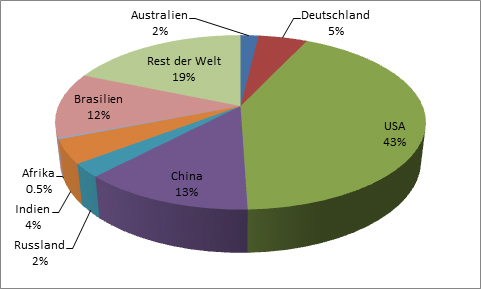
\includegraphics[width=0.8\textwidth]{images/global_revenue_share.jpg} 
 \newline
\item {Deutschland}

Das Wachstum des deutschen IT-Consulting ist mit 8,4\% sehr hoch im Verhältnis des Wirtschaftswachstums von 3\% in 2011.\cite{statGer2} Dabei haben die Top 25 IT-Consulting Unternehmen sogar noch ein größeres Wachstum mit Spitzen bis zu 10\%. \cite[6]{topITB} Dies sind durchaus überdurchschnittliche Wachstumsraten, welche international mit aufsteigenden Ökonomien wie Indien, Russland oder China sehr gut mithalten können. Der Gesamtumsatz des IT-Consulting beträgt 29,4 Milliarden Euro.  Das sind 1,12 Prozent des gesamten bereinigten Bruttoinlandproduktes. \cite{statGer} Um die Dichte des IT-Consultingmarktes einschätzen zu können macht es Sinn den Gesamtumsatz auf die Ländergröße zu beziehen. 
Deutschland schneidet hier mit 8,24 Milliarden Euro pro 100000 km² ab. Dies ist im Verhältnis mit anderen Ländern eine recht hohe Dichte und bietet daher Wegersparnisse und Kommunikationsvorteile die sich strategisch günstig auswirken können.
 \newline
\item {USA}

Die USA zweifellos einen gigantischen Marktanteil an IT-Services. Mit 244 Milliarden Euro, was 43\% des weltweiten IT-Service Markt einnimmt, ist es mit Abstand das umsatzstärkste Land der Welt im Bereich IT-Services. \cite{ibisUSA} Das Wachstum stagniert allerdings mit 2,2\%. Im Verhältnis zum Wachstum des bereinigten Bruttoninlandprodukt von 1,8\% wächst es nur wenig mehr. \cite{statUSA} Die Umsatzdichte beträgt 2,48 Milliarden Euro pro 100000 km². Im Verhältnis zu anderen Ländern, ist dies eine sehr hohe Dichte und schneidet damit hinter Deutschland und weit über die anderen Länder ab.
Ein Großteil der Umsätze in den USA entsteht unter anderem dadurch, dass Wertschöpfung durch IT-Services, die im Ausland durch Offshoring entstehen, hinzugerechnet werden. Diese Offshoring-Länder sind daher ein Schlüsselfaktor für die großen Umsätze in den USA. (Siehe x.x)

 \newline
  \newline
\item {China}

China hat mit 72,6 Milliarden Euro den zweitgrößten Marktanteil der Welt. Zwar noch weniger als ein drittel gegenüber den USA, jedoch verzeichnet es mit 6,8\% in 2011 überdurchschnittliche Wachstumsraten im Bereich IT-Services und damit hat damit das dreifache Wachstum des Konkurrenten USA.  Im Verhältnis zum  Wachstum des Bruttoinlandproduktes mit 9,2\% in 2011 ist dies jedoch verhältnismäßig wenig. Es deutet stark hier daraufhin, dass die strategische Ausrichtung der IT und deren Prozessen noch nicht  gleichermaßen Beachtung geschenkt wird, wie anderen Dienstleistungen. Mögliche Ursachen könnten Fachkräftemängel oder Kostendruck sein. Es gilt daher weiter zu untersuchen, welche Ursachen das verhältnismäßig schwache Wachstum hat. Die Dichte ist im Verhältnis zu Deutschland oder den USA auch sehr schwach. Hier schneidet China mit einer IT-Service-Dichte von 0,74 Milliarden pro 100000 km² ab. Da China sehr weitläufig und nicht vollständig industrialisiert ist, ist diese Größe wenig aussagekräftig und es besteht weiterer Untersuchungsbedarf, ob dies wirklich auf eine schwache Entwicklung hindeutet oder anderen demografischen Umständen geschuldet ist \cite{ibisChina}
 \newline
 \newline
\item {Russland}

Der russische Markt im Bereich IT-Services ist mit 14,3 Milliarden recht klein wenn man es auf die Größe des Landes bezieht. Es gibt vor allem viel Systementwicklung und hardwarenahe Entwicklung. Dienstleistungen im IT-Sektor wachsen jedoch in zunehmenden Maße und konnte 2011 15,3 Prozent Branchen-Wachstum erreichen. Dies ist sowohl im internationalen als auch im Verhältnis zum Wachstum des Bruttoinlandproduktes mit 4,3 \% in 2011 weit überdurchschnittlich. \cite{statRus2} Aufgrund der relativ kostengünstigen Entwicklungkosten für Software, insbesondere hardwarenahe Entwicklung und Systemengeneering wird Russland vor allem in Europa  zunehmend als „Offshoring Land“ attraktiv. (Wirtschaftsinformatik und Management 12/2013, Offshoring Land Russland)
Die Dichte des IT-Consulting fällt mit 84 Millionen Euro pro 100 000 km² sehr niedrig aus. Dabei ist zu berücksichtigen, dass ein Großteil von Russland gar nicht oder nur schwach bewirtschaftet ist. \cite{statRus}

 \newline
 \newline
\item {Afrika}

Afrika hat einen sehr niedrigen Anteil am Markt mit 1,4 Milliarden. \cite{statAfr} Statistiken zum Wachstum konnten leider nicht gefunden werden. Die großen Technologie-Beratung-Konzerne haben sich in verschiedenen Teilen Afrika als Beratungen etabliert, die auch den IT-Consulting Markt abdecken. Der Trend geht jedoch laut Experten immer mehr dahin, dass neue inländische IT-Service-Provider auf dem Markt konkurrieren und die US-Konzerne ablösen. Afrika hat 2011 mit 5\% ein durchaus gutes Wirtschaftswachstum zu verzeichnen, kann aber nicht mit anderen aufstrebenden Ökonomien mithalten, insbesondere nicht im IT-Umfeld. \cite{statAfr2}
Ursachen liegen hier nicht zuletzt in der Stromversorgung. Denn 80\% der Dörfer in Afrika sind immernoch ohne Stromversorgung, weil Energieanbietern die Vernetzung der Dörfer zu teuer ist.  \cite{dieZeit}
Die demografische Lage im gesamten Kontinent zu betrachten ist jedoch sehr vielschichtig. Eine Analyse des Marktes in sehr komplex, da dort sehr viele demografische Umbrüche stattfinden. Daher ist hier eine Betrachtung der Umsätze wenig aussagekräftig für eine klare Einschätzung. Es besteht daher hier weiterer Forschungsbedarf, um die Kennzahlen in einem differenzierteren  Kontext zu stellen.

 \newline
 \newline
\item {Brasilien}

Brasilien hat in 2011 mit einem Branchenumsatz von 69,6 Milliarden den drittgrößten Anteil am IT-Consulting Markt. Das Wachstum über die Jahre von 2008-2011 beträgt 61\%. \cite{statBras2} Trotz seiner flächenmäßigen Größe weist es dadurch mit 0,82 Milliarden pro 100 000 km eine verhältnismäßig hohe Dichte auf. Der Wachstum in 2011 in der IT-Services-Branche beträgt hier 4,9\% und ist damit weitaus höher als das Gesamtwirtschaftswachstum mit 2,7\%. Dabei beträgt der Anteil am Bruttoinlandprodukt allein 4,5\%. Dies zeigt welchen großen Stellenwert der Markt für IT-Services in Brasilien einnimmt. Experten prognostizieren weiterhin einen rasanten Anstieg des Wachstums, insbesondere im Bereich BPO, welche laut Schätzungen 85\% am Gesamtmarktanteil einnimmt.\cite{statBras}


\end{itemize}



\section{Arbeitskultur}
	\subsection{Einleitung}
Bevor die Wichtigkeit der Arbeitskultur für die Beratungsdienstleistung erläutert wird, wird an dieser Stelle auf die Definition der Arbeitskultur eingegangen. Reinhard Kößler definiert den Begriff der Arbeitskultur im ``Lexikon zur Sozialogie`` von Wernern Fuchs-Heinritz als Verschiedenheit von Visionen des Arbeitsverhaltens in Form von Lebensformen, Einstellungen und Reaktionen auf die Anforderungen der Arbeit in industriell-kapitalistischen Gesellschaft. \cite{Fuchs-HeinritzLautmannRammstedtWienold1994}.
Arbeitskultur ist in der ersten Linie eine Teilmenge der Kultur (Sitten, Bräuche, Mentalität usw.) einer Nation. Gemäß Carsten Weigelt bedeutet die Arbeitskultur für die jungere Generation - sogenannten ``Digital Natives`` viel mehr als Geld und Karriere. Unter Arbeitskultur wird von ihnen das Wohl im Privatleben und am Arbeitsplatz verstanden.\\ Die Arbeitskultur gehört zum Beratungsprozess und spielt dabei nicht die unwesentlichste Rolle. Welche Arbeitskultur gehört zum Beruf des IT-Beraters? Ein IT-Berater ist immer in der Bewegung und sein Arbeitsplatz ist nicht nur im Büro sondern auch im Zug, im Restaurant oder im Auto. Es ist sehr ersichtlich, dass die Arbeitskultur des Beraters mit der Arbeitskultur von Kunden des Beraters unzertrennlich ist. IT-Consultans kennen innerhalb der wenigsten Zeit sehr viele Firmen und deren Mitarbeiter lernen. An dieser Stelle stoßen die IT-Berater auf unterschiedlichsten Arbeitskulturen auf. Berater arbeiten oft durch Kommunikation mit Menschen aus unterschiedlichen Unternehmensebenen (Mitarbeiter, Manager, Geschäftsführer usw.), verschiedenen Branchen (Finanzdienstleistung, Fahrzeugbau, Großhandel, Chemieindustrie usw.) oder unterschiedlichen Länder mit jeweils einzigartigen Kulturen sowie Arbeitskulturen.\\
Im Vergleich zu einem Mechatroniker, der nur eine Arbeitskultur ``kennt``, konfrontieren die IT-Berater mit unterschiedlichsten Arbeitskulturen (manchmal auch international).\\
Um die Bedeutung der Arbeitskultur im internationalem Kontext für den Beratungsprozess näher zu erläutern, werden an dieser Stelle 2 Beispielfälle erklärt.\\
	 \\
	 a) Das 1. Fall ist ein IT-Consulting-Unternehmen mit eingestellten Beratern, die aus unterschiedlichen Ländern kommen, unterschiedliche Sprache sprechen und sich kulturell enorm unterscheiden. Wichtig für die Arbeitskultur an dieser Stelle ist kulturellen Gleichgewicht herzustellen und dauerhaft zu behalten. Diese Berater arbeiten zielgerichtet und ständig im Team. Im 1. Fall wird dem Autor dieser Arbeit sehr interessant, inwieweit sich kulturellen Unterschiede auf das gemeinsame Ziel des Beratungsprozesses bei der Softwareeinführung auswirken können. Auch interessant ist hier wie die IT-Berater aus unterschiedlichen Länder mit Kunden aus Deutschland umgehen, ob die kulturelle Unterschiede einen Einfluss auf Kundenbeziehungen haben oder nicht. \\
	 \\
	 b) Das 2. Fall bezieht sich auf ein deutsches Unternehmen, das sich international agiert und Kunden aus unterschiedlichen Länder betreut. In diesem Fall müssen sich deutsche Mitarbeiter auf unterschiedliche Arbeitskulturen anpassen. Denn ein Meeting während des Mittagsessen in Japan ist widersinnig und wirkt unseriös (in Japan hat das Essen einen unverletzlichen Status), in USA dagegen ist es nicht ungewöhnlich, dass beim Essen wichtige Entscheidungen kollaborativ getroffen werden.\\
	Wegen der zeitlichen sowie thematischen Begrenzung liegt der Autor dieser Arbeit den Fokus nicht auf die Differenzierung dieser zwei Fälle sowie kulturelle Unterschiede der Berater, sondern nur auf die unterschiedliche Arbeitskulturaspekte, die für den Beratungsprozess ausschlaggebend sind. Teilaspekte der Arbeitskultur, die den Autoren dieser Arbeit interessant erscheinen, werden in folgenden Kapiteln vorgestellt und verglichen. In diesem Sinne werden diese zwei Fälle nicht unterschiedlich und nur im Hintergrund behandelt.
	Diese sind aber wichtig, um zu zeigen warum die IT-Berater-Arbeitskultur nicht nur auf die deutsche Arbeitskultur sich bezieht, sondern auch im Beratungskontext einen internationalen Charakter hat.\\
	\\
\textbf{Allgemeine Arbeitsabläufe des IT-Consultings}\\ \\
	Nachdem die Arbeitskultur erklärt wurde, werden in diesem Kapitel allgemeine Abläufe des IT-Consultings detaillierter betrachtet. An dieser Stelle ist es unveräußerlich den Beratungsprozess exemplarisch zu zeigen, um die Feinheiten des Prozesses zu verstehen, die von der Arbeitskultur beeinflusst werden. 
	IT-Consulting ist eine wichtige Art des Consultings in IT-Fragen eines Unternehmens. Das Wesen des IT-Consultings besteht im Allgemeinen darin, Unternehmen bei der Neustrukturierung der Anwendungslandschaften oder bei der Pflege der bestehenden Informationssysteme zu unterstützen. Während des gesamten Beratungsprozesses bleibt Berater als externe Experte solange im Unternehmen bis die Probleme, die er mit seinem technischen Fachwissen zu lösen hat, nicht mehr existieren oder selbständig von den Mitarbeitern des Unternehmens gelöst werden können.\\
	Um den Beratungsprozess zu verdeutlichen wird jetzt ein Beispielprozess aus der Praxis der IT-Beratung beschrieben. Ein Online-Handelsunternehmen möchte ein BI-Standardsoftware einführen und die Daten für Analysezwecke aus dem bestehenden ERP-System zu laden, um die potentiellen Kündiger zu vermeiden oder neue Kunden zu gewinnen. Am Anfang jedes Prozesses muss dem Berater die Organisationsstruktur und die Geschäftsprozessabläufe des Unternehmens klar sein, um eine passende Lösung zu finden. IT-Berater haben eine Standardsoftware im Einsatz, um geschäftlichen Probleme eines Unternehmens mit Hilfe von Informationstechnologie zu lösen. Es gibt aber keine Standardlösung die für alle Unternehmensstrukturen passend ist, weil die Unternehmensstrukturen meistens heterogen sind. Nach dem erfolgreichen Vertragsabschluss zwischen Unternehmen und der Consultingfirma beginnt die Analysephase des Beratungsprozesses. Hier wird die Unternehmensstruktur des Online-Handelsunternehmen analysiert, bis man erkennt wo die Software eingesetzt werden kann, Stellen wo die Reibungen entstehen können, welche Ressourcen stehen zur Verfügung und welches Informationssystem sich am besten für den Unternehmenszweck eignen kann. Es muss ständig ein Feedback zwischen dem Berater und Unternehmensführer oder dem Projektleiter durchführbar sein.\\
	Jetzt wird der Ablauf des Beratungsprozesses intensiver beschrieben. Nach der Analysephase beginnt man der Konzepterstellung indem für die Ideen und Pläne ein geeignetes Konzept erstellt wird. In der Folge beginnt die Umsetzungsphase, dadurch eine neue IT-Architektur aufgebaut oder die vorhandene ergänzt wird. Im unseren Beispiel wird die ERP-Lösung mit der BI-Lösung erweitert, die vorhandene Architektur bleibt erhalten. In dieser Phase können auch die andere Berater aufgerufen werden, falls es viele komplizierte Realisierungsmaßnahmen gibt.
	Nachdem das Informationssystem erfolgreich in die Unternehmensstruktur integriert ist, beginnen die Schulungsmaßnahmen, damit die Mitarbeiter des Unternehmens in der Lage sind mit diesem System umgehen zu können. Zum Schluss erfolgt die Wartungsphase und Intensität der Beratungsdienstleistung nimmt langsam ab. Diese Prozesskette kann in Form eines Lebenszyklus stattfinden.\\
	Diesen Ablauf kann man graphisch am folgenden Modell des ganzheitlichen Beratungsprozesses erkennen(seih Abb. 4.3). Dieses Modell liefert uns die einzelnen Phasen der Beratungsdienstleistung eines Freelancers im Gebiet der Managementberatung \cite{MngmBerPhasen}.


\begin{figure}[htp]
\centering
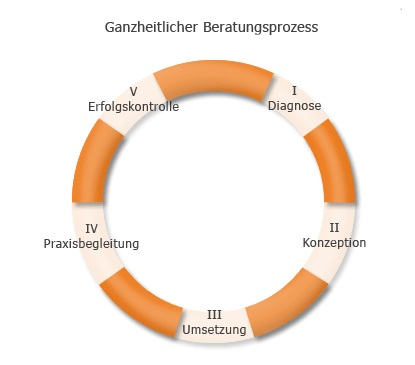
\includegraphics[width=0.7\linewidth]{./images/beratungsproz}
\caption{Phasen des Beratungsprozesses  eines Managementberaters, \cite{PhasenBeratungsprozess} }
\label{fig:beratungsproz}
\end{figure}
	
	\textbf{ Bedeutung der Arbeitskultur für IT-Consulting}\\ \\

	In wie weit ist es wichtig die Arbeitskultur für den Beratungsprozess zu betrachten? Anhand vom unseren Beispiel ist es zu erkennen, dass die IT-Berater in jeder Phase der Softwareeinführung mit den Unternehmensvertretern kommunizieren sollen. Es ist wichtig, dass die Berater genug technisches Know-how mitbringen, noch wichtiger sind die Soft Skills, die für erfolgreiche Geschäftsbeziehungen entscheidend sind. ``IT Business is People's Business``. Damit wird gemeint, dass der Erfolg von   IT-Projekten sowohl auch von den vertrauensvollen Verhandlungen maßgeblich von der Kompetenz des Beraters abhängt. \cite{ITConsRu}
	Welche Social Skills des IT-Beraters sind für Deutsche als obligatorisch nötig? Sind diese persönlichen Eigenschaften auch für die anderen Nationen von der Bedeutung? Unternehmensführung und IT-Berater müssen bei der Lösung des Problems einig werden. Der Berater muss ein Unternehmen für seine vorgeschlagene Lösung überzeugen. Muss man, um das Unternehmen zu überzeugen, nur eine gute Software anbieten und als vertrauenswürdiges Unternehmen am Markt agieren oder reichen diese Bedingungen beispielsweise in Indien nicht aus, weil der Berater möglicherweise aus anderer Kaste ist. Denn die Kastenzugehörigkeit hat in Indien bis heute kulturelle und soziale Auswirkungen auf viele Lebensbereiche \cite{KastensystemInd}.

	Für diese Arbeit ist wichtig zu wissen wie die Arbeitskultur in ausgewählten Länder sich unterscheidet und in wie weit diese den Beratungsprozess beeinflussen kann.
	In den folgenden Kapiteln wird Arbeitskultur von ausgewählten Länder(Russland,Japan, USA, Deutschland) untersucht und zum Schluss werden einige interessanten Fakten verglichen und diskutiert. 
\subsection{Teilaspekte}
	In diesem Kapitel werden die Teilaspekte von ausgewählten Ländern vorgestellt. Einige Teilaspekte werden detaillierter beschrieben, um die Wichtigkeit dieser Aspekte für das IT-Consulting hervorzuheben. Für die bessere Übersicht, um die die Teilaspekte in ausgewählten Ländern zu vergleichen, wird eine Matrix aufgestellt. Die Felder dieser Matrix bleiben zuerst leer und nach dem die einzelne Aspekte von den Ländern recherchiert und vorgestellt werden, wird die Matrix noch mal mit den ausgearbeiteten Feldern ausgefüllt. Die Recherche findet in 3 Sprachen (Deutsch, Englisch und Russisch) statt, um den Fokus der Recherche zu verbreiten.
	
\begin{table}[htp]
\begin{tabular}{|c|c|c|c|c|c|}
\hline  Aspekt/Land& Deutschland & USA & Russland & Japan & Indien \\ 
\hline 	Hierarchien  & ? & ? & ? & ? & ? \\ 
\hline  Kundenverhältnisse& ? & ? & ? & ? & ? \\ 
\hline  Gesetze& ? & ? & ? & ? & ?  \\ 
%\hline  Grad des intuitiven Handelns& ? & ? & ? & ? & ? & ? \\ 
\hline  Kritikfähigkeit& ? & ? & ? & ? & ? \\ 
\hline  Team& ? & ? & ? & ? & ?\\ 
\hline  Entscheidungsfindung& ? & ? & ? & ? & ?  \\ 
\hline  Lebensstandard& ? & ? & ? & ? & ? \\ 
\hline  Pünktlichkeit& ? & ? & ? & ? & ?\\ 
\hline  Arbeitszeit, Urlaub, W-L-B& ? & ? & ? & ? & ?\\ 
\hline 
\end{tabular} 
\caption{Matrix der Arbeitskultur}
\end{table}
%Ende der Recherche-> Information für neue Matrix
%1)Hierarchien und Organisation->Hierarchien 2)Kundenverh weg 3)spezielle Rechtslage->Gesetze 4)Grad des intuitiven Handelns weg 5) Kritikfähigkeit nur bei Japan,De 6) Lebensumstände ->Lebensstandards ->Zeitmanagement in Form von Pünktlichkeit 7)Work-Life-Balance-> Arbzeit und Urlaub 8)Entsch.findung nur Russland
%
%Durch einer Recherchewerden einige Teilaspekte verändert. Dafür gibt es mehrere Gründe, bspw. waren die recherchierten Teilaspekte besser formuliert oder einige waren in ihrer Definition zu weit gefasst und müssten demzufolge zusammengefasst werden. Für bestimmte Teilaspekte gibt es keine Information, die durch Recherche in 3 verschiedenen Sprachen (Deutsch, Englisch und Russisch) nicht zu finden ist. An dieser Stelle besteht noch Forschungsbedarf. 
Dieses Kapitel hat im Vergleich zu den Kapiteln ``Markt`` und ``Bildung`` eine andere Struktur, indem nicht nach den Teilaspekten der Arbeitskultur gegliedert wird. Dafür wird hier eine Unterteilung des Kapitels nach Ländern vorgenommen und in diesen werden die Teilaspekte wie Hierarchien, Gesetze oder Team beschrieben.
Bevor die ausgewählten Ländern untersucht werden, definiert man in folgenden Kapiteln zuerst die wichtigsten Teilaspekte der Arbeitskultur.

\subsection{Analyse der ausgewählten Teilaspekte}

	\subsubsection{Russland}

	
	\textbf{Einleitung}\\ \\
	Der Aspekt-Markt spielt für die Arbeitskultur nicht die unwesentlichste Rolle. Zwischen diesen Aspekte gibt es einige Zusammenhänge wie das Gehalt oder die Arbeitszeiten von IT-Berater.\\
	Russland ist ein Wachstumsmarkt mit Zukunft. Laut Holger Hirsch ist heute der damals geschützter russischer Markt offen für Exporte und Investitionen aus Deutschland. Dies gilt sowohl für IT-Beratungs-Unternehmen, die ihre Softwareprodukte in Russland integrieren auch für russische Manager, die bei der Informationstechnologie auf westliches Know-how setzen.\cite{ITConsRu}\\
	Da der Markt für IT-Beratung neu ist, muss man als IT-Berater aus Westen ganz viele Entscheidungen intuitiv treffen. Hier weden natürlich die Soft Skills des Beraters gefragt. Technische Fähigkeiten, funktionales Wissen und Branchen-Know-how sind selbstverständlich vorausgesetzt. Sonst wären die höheren Gehaltstarife für westlichen Berater ungerechtfertigt. Mit anderen Wörtern müssen deutsche Beratern ein breiteres Wissen besitzen als ihre russischen Kollegen, um möglicherweise an den russischen Softwareprojekten teilnehmen zu können. ´´Der Zerfall der Sowjetunion und die Reformen im wirtschaftlichen und sozialen Gefüge Russlands haben einen erheblichen Einfluss auf die Arbeitskultur in gegenwärtigen russischen Organisationen´´\cite{ProzessbeglBerRU}.
	Deswegen überlappen sich die kulturelle mit reformbedingten Faktoren der Arbeitskultur. Es ist daher sehr schwer den Ursprung dieser Faktoren zu unterscheiden. Am Beispiel des russischen Kollektivs könnte diese Überlappungen der russischen Kultur und sowjetischen Reformen ersichtlich werden. Autor dieser Arbeit möchte an dieser Stelle auf Beschreibung von Teilaspekten der Arbeitskultur eingehen und nicht auf die detaillierten Erklärungen von den Ursachen der Entstehung der Teilaspekte, solange es nicht im Kontext des IT-Consultings relevant ist.\\ \\

	\textbf{Gehalt}\\ 
	\\
	Der russischer Senior-Consultant aus Moskau verdient im Mittel 3845 € im Jahr. Das ist für russische Verhältnisse relativ hoher Gehalt. Zum Vergleich beträgt der durchschnittlicher Gehalt in Russland beim aktuellen Währungskurs 587,60 €(in Moskau 927.57 €) \cite{RusGehAllgm}. Es gibt  in Russland sehr starke regionale Gehaltsunterschiede. Aus dem unten stehenden Diagramm kann man den Unterschied des monatlichen Gehalts für SAP-Berater ermitteln. Im Großen und Ganzen verdient man in beiden Metropolen Moskau und Sankt-Petersburg ca. das doppelte wie in anderen Großstädten wie Rostov, Wolgograd oder Omsk.
	\\
\begin{figure}[htp]
\centering
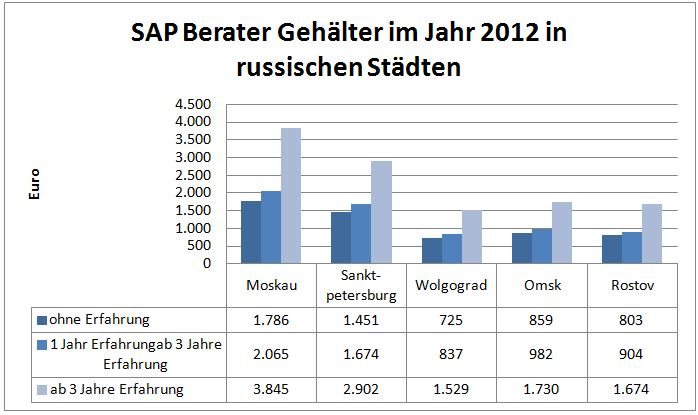
\includegraphics[width=0.7\linewidth]{./images/SAP-Berater_Gehalt_RU}
\caption{SAP-Berater Gehälter in Russland \cite{GehaltSAPBerRU}}
\label{fig:SAP-Berater_Gehalt_RU}
\end{figure}
\\
%Quelle:http://www.tadviser.ru/index.php/%D0%A1%D1%82%D0%B0%D1%82%D1%8C%D1%8F:%D0%A0%D1%8B%D0%BD%D0%BE%D0%BA_%D1%82%D1%80%D1%83%D0%B4%D0%B0_%D0%B2_%D0%A0%D0%BE%D1%81%D1%81%D0%B8%D0%B8_(%D0%98%D0%A2_%D0%B8_%D1%82%D0%B5%D0%BB%D0%B5%D0%BA%D0%BE%D0%BC)
	Senior IT-Berater aus Deutschland verdient zum Vergleich durchschnittlich 6.250 € im Monat\cite{GehaltSAPBerDE}. Die deutschen Berater, die nach Ausland geschickt werden, haben noch höheren Gehaltstarif. Der Junior Berater im IT Umfeld ohne Projekterfahrung  verdient in Russland durchschnittlich 1200 € monatlich\cite{GehaltSAPBerRU}. Laut der russischen Arbeitsagentur ``rabota.ru`` steigt die Anfrage auf ERP-Systemen enorm und deswegen steigen auch die Gehälter für Spezialisten in diesem Umfeld. Die Anfänger im IT-Beratungsbereich sind bereit am Anfang der Karriere fast kostenlos zu arbeiten, um Gold werte  Erfahrungen im ERP-Bereich zu sammeln \cite{RusGehRabota}.
	Der deutsche Junior-Berater mit den gleichen Qualifikation und Erfahrung verdient ca. drei mal so viel (3750 €) \cite{GehaltSAPBerDE} als sein russischer Kollege.\\ \\
	\textbf{Team: %und Organisation: 
	Russischer Arbeitskollektiv gegen westlichen Team}\\
	\\
	``Das Arbeitskollektiv wurde in der sowjetischen 
	Epoche als das zentrale soziale Handlungsfeld propagiert. Es repräsentiert,dass die Geschlossenheit der Gruppe wichtiger als die Selbstverwirklichung der einzelnen Gruppenmitglieder`` ist.\cite{ProzessbeglBerRU}\\
	Gruppeninterne Konflikte wurden deshalb weniger vermieden oder nicht diskutiert. Der Unterschied gegen dem westlichen Team besteht darin, dass russischer Kollektiv eine dauerhafte Einrichtung mit klar zugewiesenen Leitungskompetenzen ist, die vom Vorgesetzten häufig ausgeübt werden. Im Gegensatz zum russischen Kollektiv wird das westliche Team nur für die Dauer eines bestimmten Projektes eingerichtet und zeichnet sich durch die Gleichberechtigung aller Teammitglieder aus.\\
	So ein Kollektiv für Beratungszwecke ist demzufolge oft nicht flexibel und ist zu stark weisungsgebunden. Die Aufgaben im Kollektiv werden meistens vom Vorgesetzten vorgeschrieben, im unser Fall von einem Projektleiter oder einem Manager. Solche Führungspersonen sind im IT-Beratungsfall oft an dem Büro gebunden und sind meistens in diesem Büro während die Berater oft unterwegs bei den Kunden sind. Daher müssen die Entscheidungen intuitiv und unabhängig von dem Vorgesetzten getroffen werden. Die Tatsache, die Entscheidungen intuitiv zu treffen, spiegelt sich dem Prinzip des russischen Kollektivs wieder.  ``Russische Organisationen zeichnen sich durch eine Konzentration von Macht auf die Führungskräfte aus. Ohne den Vorgesetzten werden keine Entscheidungen getroffen``. \cite{ProzessbeglBerRU} \\
	Verlagerung von Entscheidungen auf die Mitarbeiter wird in Russland selten stattfinden, deswegen werden die Mitarbeiter von den Führungskompetenzen befreit und übernehmen oft nur Ausführungsanweisungen. Für  den Beratungsprozess ist diese Tatsache ein reisen Minuspunkt, weil die Berater das interdisziplinäres Wissen besitzen und  den vollen Handlungsspielraum in der IT-Beratungsszene brauchen.
	Zu erwähnen wäre noch, dass die jungen Menschen von solcher Stereotypen weiter entfernt sind als die ältere ``sowjetische`` Generation. \\ \\
	\textbf{Gesetze: Personalauswahl und russische Gesetze}\\
	\\
	 Eine weitere wichtige Besonderheit ist die Personalauswahl. Häufig erfolgt die Auswahl von neuen Mitarbeitern nicht nach Kriterien der fachlichen Kompetenz. Oft werden Arbeitsplätze unter Verwandten und 
	 Freunden vergeben. Es existieren fast keine etablierten Mechanismen von Angebot und Nachfrage auf dem Arbeitsmarkt. Vakanzen werden häufig nicht an den fachlich geeignetsten Bewerber vergeben, sondern an ``unseren Mann``(nash chelovek). Sinngemäße Übersetzung bedeutet, dass ``Unser Mann`` oder ```nash chelovek`` eine besondere, meist verwandtschaftliche Beziehung zum Unternehmensführer oder den Vorgesetzten des Unternehmens hat.\\
	 Ein weiteres für russische Arbeitskultur typisches Merkmal ist, dass die Gesetze, Bestimmungen und Regelungen keinen eindeutig verbindlichen Charakter haben. In Abhängigkeit von der Situation und den involvierten Personen, können Regeln oder Gesetze bewusst unberücksichtigt bleiben. Wie sich jedoch diese Abstufung darstellt ist nicht vorhersagbar. Das liegt auch daran, dass das russische Volk und die russischen Behörde sich einander nicht zutrauen. Die Strenge des Gesetzes wird oft in der Vernachlässigung der Gesetzgebung ausgeglichen. \cite{ProzessbeglBerRU}\\ \\ 
	 \textbf{Arbeitszeit, Urlaub, Work-Life-Balance}\\ %Work-life-Balance gehört dazu
	 \\
	 Die gesetzliche Wochenarbeitszeit in Russland beträgt 40 Stunden. Doch in meisten Fällen wird diese Grenze total überschritten. Die IT-Spezialisten arbeiten zwischen 10 und 11 Stunden am Tag in einem 5-Tage-Rhythmus \cite{ArbZeitRU}. 
	  Oft wird auch eine 6-Tage-Woche praktiziert. Zum Vergleich arbeiten deutsche IT-Berater oft weniger (sieh Kapitel-Deutschland ``Arbeitszeit und Urlaub``) und die wöchentliche Arbeitszeit der japanischen Kollegen(sieh Kapitel-Japan ``Arbeitszeit und Urlaub``) ist am längsten in den ausgewählten Ländern. 
	 In vielen Tarifverträgen in Deutschland beträgt der Jahresurlaub 30 Arbeitstage. In Russland sind es dagegen nur 24 Tage. Der Arbeitstag beginnt bei russischen nicht produzierenden Firmen um 9 oder 10 Uhr \cite{ArbZeitRU}. Wenn ein IT-Berater um 10 Uhr mit seiner Arbeit beginnt, dann ist er vermutlich um 20-21 Uhr zu hause. Daraus lässt sich schlussfolgern, dass es aufgrund der Zeitmangel auf die persönliche Bereiche wie die Freunde, Familie und Work-Life-Balance von russischen Beratern eine negative Auswirkung gibt.   \\ \\
	 \textbf{Pünktlichkeit und Reisen }\\
	 \\
	 Der IT-Berater-Beruf ist eine Tätigkeit, die mit höheren Reisebereitschaft verbunden ist, Beratung heißt meist, beim Kunde vor Ort zu sein. In Deutschland sind die Berater ganz oft mit Autos unterwegs. Von einem deutschen Großstadt bis zum anderen braucht man beispielsweise 4-5 Stunden. In Russland gibt es 2 grundsätzliche Transportprobleme mit dem Consulting-Hintergrund, die dem Autor auf den Ersten Blick erscheinen: Staus in Moskau und große Entfernungen zwischen den russischen Städten. Nachfolgend wird der Autor diese 2 Probleme näher erläutern. Das Land ist sehr groß und weit (es umfasst 11 Zeitzonen).
	 Zwischen Moskau und Nowosibirsk sind es ca 4 Stunden nur Flugzeit plus 3 Stunden Zeitunterschied. Wenn ein Berater aus Moskau seinen Arbeitstag am Montag in Nowosibirsk beginnen möchte, muss er schon am Sonntag ausreißen. Die Reisen sind erschöpfend und könnten von russischen Berater,die eine Familie haben, nicht so gern angenommen. Für diese Familienleute stören auch die Work-Life-Balance von IT-Beratern, weil die Reisen direkt ins Privatleben eingreifen und sehr viel wertvollen Zeit kosten.\\
	 Laut dem russischen Rating "Consulting research" aus 21 größten IT-Consulting-Unternehmen befinden sich 13 Unternehmen in Moskau\cite{RaitConsRU}.
	 Aus 100 größten russischen IT-Unternehmen befinden sich in Moskau 71 Firmen \cite{100BigITConsURU}. 
	 Moskau ist nicht nur ein teuerster Hauptstadt der Welt und ein wirtschaftliches Zentrum des Landes, sondern auch ein strategisches Standort für IT geworden.
	 Mit der Stadtwachstum werden die Staus länger und länger.``Nach Angaben des GPS-Navigationsanbieters TomTom ist Mosaku Nummer eins unter den schlimmsten Stau-Städten der Welt\cite{MoskauStau1}.``
	 Da die Berater öfters unterwegs sind, ist es eine große Anstrengung in Moskau Auto zu fahren. Um von A nach B zu kommen wird ganz oft ein Metro benutzt. 
	 Deswegen ist es in Moskau ``erlaubt`` dem Berater sowie allen Geschäftsleuten ein Viertel bis halbe Stunde zum Meeting oder zum  Kunde zu spät zu kommen. Oft werden Staus als Ausrede, die auch akzeptiert wird, genutzt.\\
	 Allgemein zählt die Pünktlichkeit nicht zu den Stärken von Russen: die Termine werden nicht immer eingehalten, E-Mails werden nicht sofort beantwortet und die Versprechungen sind nicht immer realistisch. Deswegen muss man als Berater diese Verzögerungen mit einplanen \cite{RusKnigge}.\\ \\
	 	 \textbf{Hierarchie und Entscheidungsfindung}\\
	 	 \\
	 Im Teilaspekt Organisation hat der Autor erwähnt ,dass in russischen Organisationen der Chef oder sogenannte Generaldirektor  allein das Sagen hat. So beschreibt auch der Sergey Frank, dass die Entscheidungskompetenzen in Russland nicht wie gewöhnt nach unten gehen, sondern nur der Geschäftsführer die Entscheidungsbefugnisse hat \cite{RuSFI}.
	 Deswegen kommunizieren die russische IT-Berater oft nur mit dem Geschäftsführer des Unternehmens, was natürlich zur zeitlichen Verzögerungen im Projekt führen kann.\\
	 Gemäß ``Russland-Knigge`` \cite{RusKnigge} werden oft die Hierarchien in Russland nicht eindeutig und nicht klar erkennbar. Die Berater müssen schon vor Beginn der Verhandlungen herausfinden, wer das entscheidende Wort hat. Damit wird keine Zeit durch unnötige Gespräche mit Personen, die möglicherweise keinen Einfluss auf den Verhandlungsverlauf haben, verloren.\\
	 Laut ``Businessknigge Russland`` sind ``die Flache Hierarchien nicht die Sache der Russen`` \cite{RusKnigge}. Es heißt, dass auf der Ebene in der Geschäftsstruktur unter dem Unternehmensführer  sehr viele anderen Personen sein könnte, die einerseits zum Geschäft gehören, anderseits ist die Zusammengehörigkeit dieser möglichen Personen zum Geschäft sowie deren Aufgabengebiet meistens nicht klar definiert ist. An dieser Stelle in der Unternehmensstruktur könnte oben beschriebener ``nash chelovek`` auftauchen.
	
	\subsubsection{Japan}
	\textbf{Pünktlichkeit, Kritik und Besonderheit der Kommunikation}\\
	\\
	Im Geschäftsleben sind die Japaner besonders pünktlich. Pünktlich bedeutet in diesem Fall 5 bis 10 Minuten vor einem Termin zu erscheinen. Selbst nur bei 5 Minuten Verspätung müssen Sie an Ihren Geschäftspartner Bescheid geben, dass Sie sich verspäten. \cite{JPKnigge}. \\
	Die Kritik wird in Japan nicht direkt, sondern ausweichend und über den ``Umweg`` geäußert. Diese Kritikäußerung-Strategie wird auch von ausländischen Geschäftspartner erwartet. Eine Besonderheit in Japan hat die Bedeutung des Wortes ``Ja``: in einem Gespräch reagiert man mit ``Ja`` nicht auf die Zustimmung mit der Sache, sondern auf die Bestätigung des Zuhörers \cite{JPKnigge}. Ein lang-gesprochenes ```Ja`` bedeutet die Zustimmung vom bestimmten Sachverhalt.\\
	\\
	\textbf{Hierarchie und Rangordnung}\\
	\\
	Im japanischen Geschäftsleben spielt die Rangordnung eine wichtige Rolle.
	Beim Essen sitzt die wichtigste Person in der Mitte der Reihe, je größer die Entfernung von ihr, desto geringer der Rang \cite{Business-KniggeFernost}.	
	Beim Meeting wird der Ranghöchster zuerst sprechen. Bei der Begrüßung wird zuerst die Hand nicht der Frau gegeben wie das in Deutschland üblich ist, sondern dem Ranghöchsten. \\
	\\
	\textbf{Arbeitszeit, Urlaub, Work-Life-Balance}\\
	\\
	Offiziell gilt in Japan 40-Stunden-Woche, in der Realität sind Angestellten bis 21 oder 23 Uhr im Büro. Wenn jemand eher nach Hause geht als sein Chef, muss bei der nächsten Beförderung mit Konsequenzen rechnen \cite{ArbZeitJP}. Den Arbeitsplatz eher als der Chef zu verlassen zählt in Japan zu den schlechten Manieren im Geschäftsleben.
	Der Überschrift eines Online-Zeitungsartikels ``Im Japan arbeitet man sich bis zum Tode`` hat sich schon lange als Stereotyp in Japans etabliert. 
	16 Stunden am Tag im Büro, Schlafkammer, Mittagsschläfchen im Zug, unzählige Überstunden gehören zum modernen Arbeitsalltag in Japan. ``Schuld daran haben die Zeitarbeitsagenturen, denn ca ein Drittel der japanischen Arbeiterschaft besteht aus Zeitarbeitern``, sagt der amerikanische Journalist Jake Adelstein \cite{JPArbeit}. Im Gegensatz zu Deutschland, wo die Überstunden nicht immer gezahlt sind, werden in Japan die Überstunden zu der zusätzlichen Geldquelle, ohne dieser man schwer überleben kann.
	Es wurde keine Quelle gefunden, um die Arbeitszeit der IT-Berater zu bestimmen. Da kann der Autor nur persönlich vorstellen, dass 4-Tage-Woche beim Kunde mit einem zusätzlichen Tag für Meetings in der Firma bei den deutschen Berater ein Paradies für japanischen Kollegen sein kann. \\
	In Deutschland genießen die Arbeitnehmer 30 Tage einen bezahlten Urlaub. In den USA beträgt Jahresurlaub rund 2 Wochen. Offiziell sind in Japan im Durchschnitt 17 Freitage gewährt, allerdings werden nur 8 Tage im Krankheitsfall in Anspruch genommen. Weil während des Urlaubs keine Lohnfortzahlung stattfindet, muss ganz oft Urlaub unter einer Krankheit ``versteckt`` werden \cite{JPArbeitSozKultur}. Denn die Abwesenheit im Krankheitsfall wird vom Unternehmen akzeptiert und Lohnfortzahlung wird geschehen.\\
	\\
		\textbf{Gesetze: Steuer und Lebensstandard}\\
		\\
		Steuern und Sozialabgaben sind in Japan niedriger als in Deutschland. Japanischer Mehrwertsteuer beträgt im Gegensatz zu Deutschland nur 10 \%.
		``Als Arbeitnehmer ist man in Firmen mit mehr als fünf Angestellten durch eine sog. Employee Health Insurance abgesichert``. Jedoch muss man 10 bis 30 Prozent der Behandlungskosten aus eigener Tasche zahlen. Die Arbeitslosenkosten übernimmt der Arbeitgeber \cite{ArbZeitJP}.
		\\Der Lebensstandard in Japan ist vergleichbar mit dem mitteleuropäischen (sieh Abb.4.4).
		\begin{figure}[ht]
		\centering
		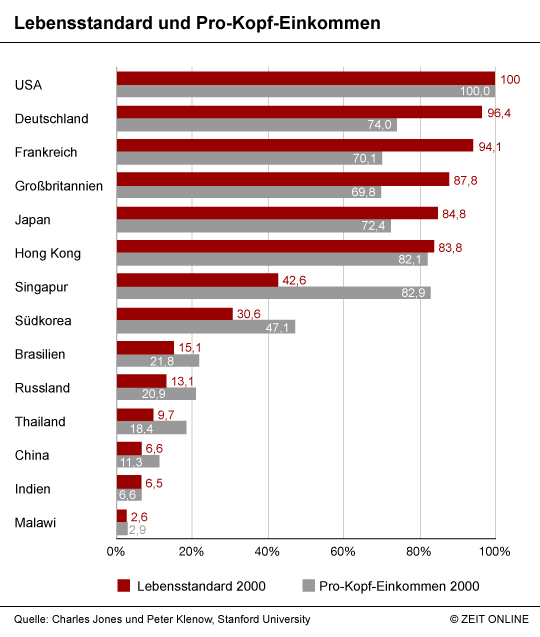
\includegraphics[width=0.7\linewidth]{./images/Lebensstandard-Pro-Kopf-Einkommen}
		\caption{Lebensstandard und Pro-Kopf-Einkommen \cite{LebensStd}}
		\label{fig:LebStdProKEink}
		\end{figure}\\
		Gemäß Miroslav Stimac sind die Ausgaben der Grundbedürfnisse in Deutschland höher als in Japan \cite[101]{Stimac2004}.
		Beispielsweise kostet Nahrung in Tokio durchschnittlich 2,36 mal mehr als in Deutschland. Viele japanische Städte leiden an Platznot, dies führt zu hohen Grundstückspreisen sowie Mietpreisen \cite[105]{Stimac2004}.
		Eine Familie mit 4 Mitgliedern im Großraum Tokio lebt oft in einer 60 qm-Wohnung \cite{ArbZeitJP}.\\	\\
		\textbf{Gehalt}\\ \\
		Einkommen in Japan hängt von dem dem Alter und der Betriebszugehörigkeit
		der Arbeitnehmer ab. Dazu kommt noch der Senioritätsprinzip, der die Gehaltshöhe dem Alter entsprechend definiert. Laut den Angaben  einer Studie der internationalen Personalagentur ``Robert Walters`` verdient ein Projektmanager in der japanischen IT-Branche rund 12 bis 17 Millionen Yen(84.000-119.000 €).
		Systemadministratoren verdienen ca 9 bis 14 Millionen Yen(63.000-98.000 €) \cite{EinkommenJP}.
		Man kann davon ausgehen, dass sich die Gehälter in der IT-Beratung auf ähnlichen oder sogar höheren Niveaus bewegen. \\ \\
			\textbf{Team}\\
			\\
		Die Bedeutung der Gruppe sowie ihr Erfolg laut Michael Gehle orientiert sich nicht auf die individuellen Ziele der	einzelnen Gruppenmitglieder, sondern auf ein gemeinsames Erfolg der Gruppe. Altruistisches Verhalten ist in japanischer Gesellschaft ausgeprägter als in Europa. Das Wohl der Einzelnen ist vom Wohl seiner Kollegen abhängig. Mit anderen Worten bedeutet dass, die erfolgreiche Zusammenarbeit der Gruppe eng an die interne Zusammenarbeit der Gruppenmitglieder angebunden  ist. Damit wird auch die Gruppe,  ähnlich wie eine Familie, die Schutzfunktion übernehmen, denn nicht nur das Erfolg des gesamten Projektes sondern auch das Risiko an die Gruppenzugehörigen zu verteilen ist \cite[233]{3LaenderVergl}.\\ \\
		\textbf{Entscheidungsfindung} \\ \\
		Im Gegensatz zu Russland werden die Entscheidungsbefugnisse auch an die untere Hierarchieebene delegiert. Damit werden auch die hohe Managementanforderungen  an die normalen Mitarbeitern gestellt \cite[233]{3LaenderVergl}.\\
		Die Japaner haben ewig lange Entscheidungswege. Die Entscheidung wird nach top-down-Methode vom Chef angestoßen, dann verläuft die Akzeptanz der Entscheidung durch eine Organisationsspirale bis jeder Mitarbeiter diese Entscheidung wahrgenommen hat. In Deutschland wird die Entscheidungen eher nach Formalismus getroffen. Innerhalb des Teams gilt eine Gleichberechtigung und der Chef hat eine Rolle des Moderators. Falls während des Projektes die Probleme aufgetreten sind, wird in Japan der Projektmanager nicht kritisiert und Schuld wird an alle Projektmitglieder verteilt. In Deutschland dagegen trägt der Projektleiter ganz oft die ganze Verantwortung für Misserfolg des Projektes.
%ab hier Korrektur
	\subsubsection{USA}
	\textbf{Team}\\
	\\
	In USA sowie in Deutschland hängt der Erfolg sowie die Karriere des einzelnen Gruppenmitglieder nicht so stark vom Gruppenerfolg wie in Japan ab. Laut Michael Gehle orientiert sich die  Karriere und Qualifizierungsmaßnahmen an einzelnen Mitarbeitern, deswegen richtet sich auch deren Verhalten eher nach individuellen und nicht nach kollektiven Zielen \cite[233]{3LaenderVergl}. 
	Teamkollegen werden in USA sowie in westlichen Ländern nicht selten als Konkurrenten angesehen, weil die Entlohnung sowie Kontrolle der Mitarbeiter an den individuellen Leistungen angehängt werden. In Japan wird dagegen durch den Sozialisationsprozess die Gruppenmitlieder eher als Familienmitglieder angesehen.\\
	 \\
		\textbf{Arbeitszeit, Urlaub, Work-Life-Balance}\\
		\\
	Arbeitszeit in den USA beträgt in der Regal 40 Stunden pro Woche. 
	Ein Drittel aller Amerikaner arbeiten länger als 40 Stunden pro Woche.
	Laut der UN-Studie arbeiten US-Angestellte im Durchschnitt etwa 500 Stunden mehr als deutsche Arbeitnehmer \cite{ArbeitsumgUSA}. Die Meisten Amerikaner haben nur 10 bezahlten Arbeitstage \cite{InfoUSArbVertr}.\\ \\
	\textbf{Gesetze: Besonderheiten in Arbeitsgesetzen}\\
		\\
		Die Lohnfortzahlung im Krankheitsfall beträgt in den USA nur 7 Tage pro Jahr. 
		Mitarbeiter im IT Bereich haben häufig keinen Anspruch auf Überstundenausgleich. Mann kann allerdings inoffiziell ein zusätzlichen Tag in der Woche frei nehmen um die Überstunden auszugleichen. Als Überstundenausgleich dient auch am Ende des Jahres ein finanzieller Bonus \cite{InfoUSArbVertr}.
		Solche Vereinbarungen sind jedoch nicht gesetzlich geregelt und müssen mündlich vereinbart werden.\\
		Die Kündigungsfrist beträgt, sowohl für Arbeitgeber als auch für 
		Arbeitnehmer, zwei Wochen. Aufgrund der kurzen Kündigungsfrist gibt es in den USA keine Probezeit.\\
		Im ersten Arbeitsjahr gibt es in den USA kein Anspruch auf Urlaub. \cite{USA_Tipps}.
		\\ \\
	\textbf{Gehalt}\\
		\\
		Laut Firma ``indeed`` beträgt ein Jahresgehalt des IT-Beraters (Technical Consultant`s in USA) rund 86.000 \$ (sieh Abb. 4.5).
		\begin{figure}[ht]
				\centering
				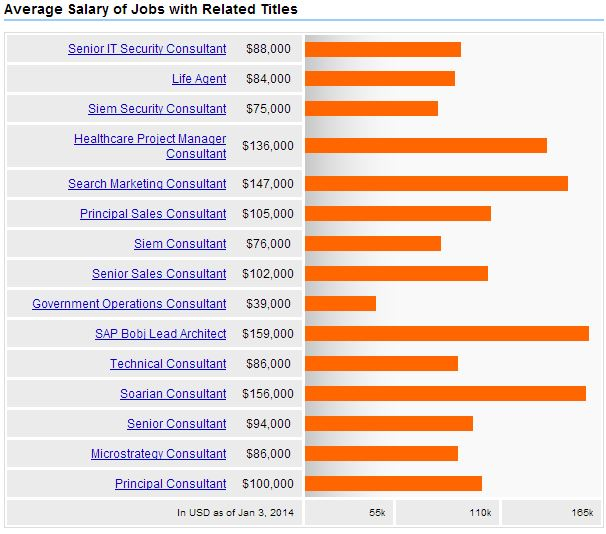
\includegraphics[width=0.7\linewidth]{./images/Techn_Cons_Sal}
				\caption{Jahresgehalt von IT-Consultants in USA}
				\label{fig:TechConsSal}
				\end{figure}\\
				%Wo ist Quelle???
		``Ein europäisches Gehalt in EUR ist ungefähr 1:1 vergleichbar mit einem 
		amerikanischen Gehalt in USD. Es wäre nicht richtig, den offiziellen Umrechnungskurs anzusetzen, da die Lebenshaltungskosten in USD in den USA mit den Lebenshaltungskosten in EUR in Europa vergleichbar sind`` \cite{InfoUSArbVertr}. In der IT-Branche wird oft ein Provision angeboten, die von erfolgreichen 
		Projekten abhängt. Das Gehalt wird in zwei Raten ausbezahlt, in der Regel am 15. und am letzten Tag des Monats.\\ \\
	\textbf{Hierarchie} \\ \\
	Gemäß US-Internetportal ``hierarchystructure.com`` \cite{HierarchieUSA} gehört die US- Geschäftshierarchie zu den erfolgreichsten Geschäftshierarchien der Welt und wird von vielen Ländern als Vorbild genommen, um das wirtschaftliche Wachstum zu erzielen. Geschäftsstruktur und Hierarchie einer Organisation werden mit dem Zweck das Gruppenziel zu erreichen aufgebaut, wobei jeder einzelne Mitglied der Organisation unterstützt wird. Dabei werden die Positionen, Aufgaben und zugehörigen Mitarbeiterrollen klar definiert.
\begin{figure}[ht]
\centering
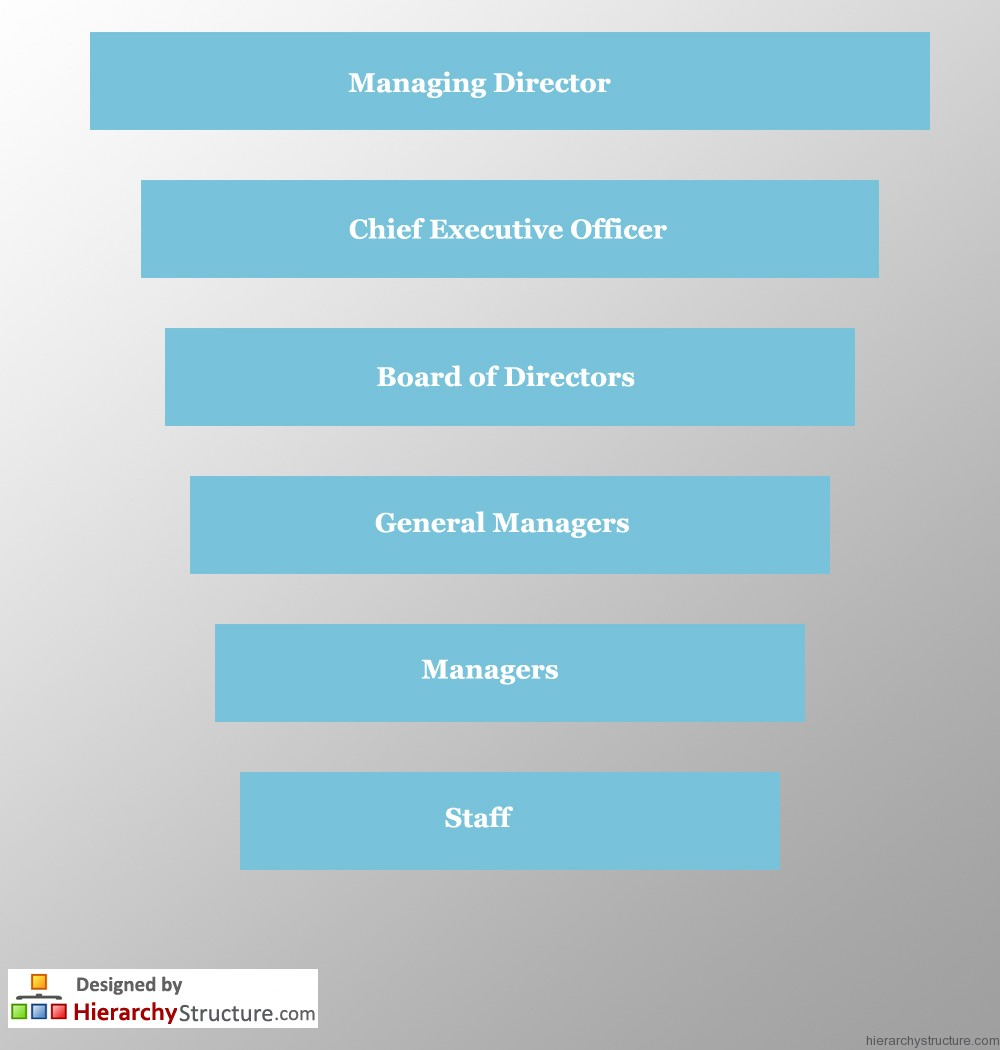
\includegraphics[width=0.7\linewidth]{./images/USA-Business-Hierarchy}
\caption{Geschäftshierarchie USA \cite{HierarchieUSA}}
\label{fig:USA-Business-Hierarchy}
\end{figure}


	\subsubsection{Deutschland}
	In allen beschriebenen Ländern unterscheidet sich erheblich der Formalisierungsgrad der Arbeitskultur. In Deutschland wird das Verhaltensweisen und Standards der Arbeitskultur sehr formalisiert in Form von gesetzlichen Vorschriften definiert. In Japan weist die Arbeitskultur auch einen hohen Formalisierungsgrad auf. Das hat nicht mit gesetzlichen Regelungen wie in Deutschland, sondern eher mit traditionellen Verhaltensweisen zu tun \cite[236]{3LaenderVergl}. Es gibt noch 2 weiteren Eigenschaften, die die deutsche Arbeitskultur bezeichnen. Dazu zählen die direkte Kommunikationsart und gründliche Planung.\\ \\
	\textbf{Pünktlichkeit}\\ \\
	Pünktlichkeit sowie gründliche Planung gehören zu den Stärken der Deutschen. IT-Consultants sind keine Ausnahme. Die Termine sollen gründlich geplant werden, bevor man zur Verhandlung kommt. Natürlich müssen die Termine zeitlich eingehaltenen werden. Es wird bei der Planung meist eine Pufferzeit eingerechnet, falls es trotz der aufwändigen Planung zu Verzögerungen kommen soll.\\ \\
	\textbf{Arbeitszeit, Urlaub, Work-Life-Balance 
	} \\ \\
	Auch die  Trennung zwischen dem privaten und beruflichen Leben zeichnet die  deutsche Arbeitskultur aus. Im Gegensatz zu China oder Russland, wo das Arbeitsteam oft als 2. Familie eingesehen ist, hat Deutschland an dieser Stelle einen formalistischen Charakter. Trotz allem was ein Team zusammen erlebt, heißen Teammitglieder unter einender ``Arbeitskollegen``. Ob diese Tatsache eine besondere Auswirkung auf Beratungsgeschäft hat, ist interessant zu wissen. An dieser Stelle besteht ein Bedarf zur Forschung.\\
	Wie schon in vorigen Kapiteln erwähnt wurde, beträgt die gesetzlich geregelte Arbeitszeit in Deutschland 40 Stunden pro Woche. Montags bis Donnerstags sind die IT-Berater oft beim Kunde vor Ort und sind zeitlich sehr ausgelastet. Das hat damit zu tun, dass die Berater, wenn sie schon beim Kunde sind, versuchen möglichst viele Probleme zu lösen. Das führt nicht selten zu den Überstunden, die am Freitag entweder durch ein Meetings-Tag im Büro oder ein Selbststudium-Tag im Home-Office kompensiert werden. Am Freitag werden beispielsweise auftretende Probleme während des Beratung analysiert und neue Lösungen vorgeschlagen. Die Work-Life-Balance, was bei vielen Unternehmen heutzutage das Modethema ist, entspricht meisten nicht den Erwartungen von den Junior-Beratern \cite{JNRBer}.\\ \\
	\textbf{Gehalt} kommt noch \\ \\
	\textbf{Lebensstandard} \\ \\
	\textbf{Hierarchie}
	
	
	
	
	

	%Quelle:Michael Gehle, Telearbeit: ein Drei-Länder-Vergleich S. 237->Tabelle!!!!!!!!!!!!
	%1)Teilaspekte umbennenen 
	%2)Deutschland
	%3)Indien?
	%\subsubsection{Indien}
	
%\subsection{Abschluss und Vergleich}
%neu Matrix-die ausgefüllt wird, mit umformulierten Teilaspekten. Begrüdnung:
%\\
%Durch einer Recherchewerden einige Teilaspekte verändert. Dafür gibt es mehrere Gründe, bspw. waren die recherchierten Teilaspekte besser formuliert oder einige waren in ihrer Definition zu weit gefasst und müssten demzufolge zusammengefasst werden. Für bestimmte Teilaspekte gibt es keine Information, die durch Recherche in 3 verschiedenen Sprachen (Deutsch, Englisch und Russisch) nicht zu finden ist. An dieser Stelle besteht noch Forschungsbedarf. \\
%1)Hierarchien->Hierarchien(plus Organisation) 2)Kundenverh weg 3)spezielle Rechtslage->Gesetze 4)Grad des intuitiven Handelns weg 5) Kritikfähigkeit nur bei Japan,De 6) Lebensumstände ->Lebensstandards ->Zeitmanagement in Form von Pünktlichkeit 7)Work-Life-Balance-> Arbzeit und Urlaub(Work-Life-Balance wird ersichtlich) 8)tagesrythmus gehört zur Arbeitszeit und Urlaub

\chapter{Bildung}
Aufgrund des wissensintensiven Charakters des IT-Consultings, ist eine hoch entwickelte Bildungs- und Ausbildungsstruktur Grundvorraussetzung für das erfolgreiche Entstehen eines IT-Consulting Marktes und für die Bereitstellung von genügend Fachkräften.
Gibt es beispielsweise nicht genügend ausreichend Ausgebildete in einem Land, aber einen hohen Bedarf an Fachkräften, müssen ausländische Mitarbeiter angeworben werden. Die Bildungssituation spielt also auch für den Aspekt Markt eine wesentliche Rolle.
Entscheidungen bei denen die Bildungssituation berücksichtigt werden muss sind zum Beispiel die Standortwahl eines Unternehmens für Expansion, Outsourcing, oder Offshoring. Auch wenn andere Firmen international übernommen werden, ist es wichtig vorher die Arbeitsmarktsituation zu betrachten. Durch Investitionen in spezielle Studiengänge, Kooperationen und Ausbildungen lässt sich langfristig der hohe Bedarf an speziell ausgebildeten Fachkräften decken. Durch die frühe Bindung an ein Unternehmen können maßgeschneiderte Mitarbeiter ausgebildet werden, die nicht erst langwierig angelernt werden müssen sondern schnell einsatzbereit sind.

Um Unternehmen angemessen beraten zu können ist auf Seiten der Consultants ein hohes Bildungslevel nötig. Dies ist erforderlich um in angemessener Zeit ein tiefes und breites IT-Fachwissen aufbauen zu können und die komplexen Zusammenhänge und Interdependenzen erkennen zu können. Dafür ist eine hohe Abstraktionsfähigkeit unbedingt nötig. Außerdem muss auch ein hohes Level an betriebswirtschaftlicher Bildung bei den potenziellen Beratern vorhanden sein oder erarbeitet werden, um die Unternehmen angepasst auf Ihre wirtschaftliche Lage beraten zu können.
Die meisten deutschen Unternehmen fordern deswegen von ihren Bewerbern einen Studienabschluss (mind. Bachelor) und teilweise technische Erfahrungen in der Entwicklung. Es existieren aber auch Länder wie zum Beispiel die Schweiz in der nur ein geringerer Teil der Schulabgänger ein Studium beginnt. In diesen Ländern reicht teilweise auch eine Ausbildung aus um trotzdem in der Consulting Branche als Bewerber akzeptiert zu werden.
Trotzdem stellt ein Studium in vielen Ländern aufgrund der wissensintensiven Tätigkeit des Beratens eine Grundvoraussetzung für diesen Bereich dar. Dabei ist natürlich zu beachten, dass die Studienqualität je nach Land und Bildungseinrichtung stark schwankt.
Im Folgenden wird zuerst eine theoretische Betrachtung zur Bildung durchgeführt. In diesem Abschnitt werden verschiedene Teilaspekte vorgestellt, die zur Bewertung der Bildung eines Landes nötig sind. Aufgrund des zeitlichen Rahmens dieser Arbeit können wird anschließend eine Auswahl dieser Aspekte getroffen und international verglichen.
 Im Abschnitt Besonderheiten des Bildungssystemes ausgewählter Länder wird auf bestimmte wichtige Besonderheiten (teilweise auch im Bezug auf das IT-Consulting) einiger Länder eingegangen. Dieser Abschnitt soll nur eine kurze Zusammenfassung einiger Besonderheiten seien, und kann das Land nicht umfassend beschreiben.
 Anschließend wird in einem weiteren Abschnitt spezieller auf die für das IT-Consulting relevante Bildung eingegangen. Diese geschieht wiederum anhand einiger ausgewählter Teilaspekte im internationalen Vergleich.


\section{allgemeine Bildungssituation}
Der Teilabschnitt allgemeine Bildungssituation beschäftigt sich mit dem Bildungsniveau in einem Land. Bildung ein sehr komplexes Thema, dass durch seine Vielschichtigkeit und die hohe Anzahl an beeinflussenden Faktoren einen einfachen Zugang erschwert. Auch die politische Situation und die Vorgeschichte eines Landes spielen eine wesentliche Rolle.

Die folgende (unvollständige) Auflistung einiger Teilaspekt soll zeigen, dass eine Vielzahl von Faktoren notwendig ist um den Bildungsstand eines Landes zu bestimmen:
\begin{itemize} 
\item Anteil der Kinder die in die Schule gehen
\item Schulpflicht
\item Alphabetisierung
\item Bildungsausgaben
\item Bildungsausgaben Anteil am GDP
\item Anzahl der Schulabgänger ohne Abschluss
\item Qualität der Bildung (PISA Studien der OECD, verschiedene Internationale Rankings)
\item Anteil der Studenten an einem Jahrgang
\item Anzahl der Absolventen in Studium und Schule im Verhältnis zur Gesamtbevölkerung
\item Anteil der Hochschulen im Vergleich zur Fläche
\item Anteil der Hochschulen im Vergleich zur Bevölkerung
\item Unterstützung des Staates (vergleichbar mit BAFöG in Deutschland)
\item ... (weitere Punkte können zum Beispiel im Bericht ``Bildung auf einen Blick' der OECD' gefunden werden)
\end{itemize}

Internationale Organisationen wie zum Beispiel die OECD (Organisation of Economic Co-Operation and Development) und die UNESO ( United Nations Educational, Scientific and Cultural Organization) haben komplexe Bewertungsverfahren entwickelt mit denen sich Bildung anhand verschiedener Indikatoren messen lässt.
Die Veröffentlichung der Unesco heißen: World Data on Education \cite{unesco2} und auf deutsch der Weltbildungsbericht \cite{unesco1}. Der Bericht von 2010 ``Reaching the marginalized'' beschäftigt sich mit der Finanzkrise und Ihren internationalen Auswirkungen auf das Bildungssystem. Die UNESCO verwendet aber oft Zusammenfassungen von Regionen der Welt (zum Beispiel Sub-Saharan Africa oder Middle East). Dadurch ist diese Ausarbeitung für eine länderspezifische Darstellung zu grob. 
Die OECD veröffentlicht jährlich einen eigenen Bericht: Education at a glance (Bildung auf einen Blick) \cite{oecd5} . Die Schwierigkeit bei dieser Veröffentlichung  besteht jedoch im Vergleich mit einigen Entwicklungsländern (zum Beispiel China und Indien), da diese nicht mit zur OECD gehören und somit nicht bewertet werden. Dieser Bericht ist aber wesentlich feiner, denn er bietet Daten für viele Länder (eben für diejenigen die zur OECD gehören). Trotzdem sind auch für die nicht enthaltenen Länder teilweise Statistiken der OECD verfügbar, zum Beispiel für Indien: \cite{oecd}, aber eben keine umfassenden Berichte.

Im Folgenden werden einige ausgewählte Teilaspekte der allgemeinen Bildung und teilweise ihre Relevanz für das IT-Consulting erläutert.

\subsection*{Anzahl der Hochschulen im Verhältnis zur Fläche (Dichte)}
Die Anzahl der Hochschulen ist für den Bereich der universitären Forschung von großer Bedeutung. Diese prägen maßgeblich die Forschungslandschaft eines Landes mit. Auch für die Ausbildungssituation ist die Anzahl der Hochschulen relevant. Denn um so mehr Hochschulen existieren, desto mehr ausgebildete Fachkräfte stehen der Wirtschaft (potenziell) zur Verfügung. 
Trotzdem ist es schwierig nur aufgrund der Anzahl der Hochschulen eine Aussage zu treffen, da dabei die Größe eines Landes außer Acht gelassen wird. Intuitiv ist klar, dass ein größeres Land (bei gleichem Entwicklungstand) im Vergleich zu einen Land das nur halb so groß ist, wahrscheinlich mehr Hochschulen besitzt. Deswegen eignet sich die „Dichte“ der Hochschulen anhand des Verhältnissen von  Fläche des Landes zu der Anzahl der Hochschulen besser als die alleinige Angabe der Anzahl.
Diese „Dichte“ besitzt jedoch auch einige Schwachstellen. So ist es mit dieser Kennzahl schwierig Länder mit großen dünn besiedelten Gebieten (z.B. Russland) mit kleinen dicht besiedelten Ländern (z.B. Deutschland) zu vergleichen. Allgemein wird einer sehr ungleichmäßigen Bevölkerungsverteilung im Vergleich zur Fläche durch dieses Verfahren keine Bedeutung beigemessen.

\subsection*{Anzahl der Hochschulen im Verhältnis zur Bevölkerung}
Diese Kennzahl ist sehr ähnlich zum oben genannten Flächenverhältnis. Durch das Verhältnis von Bevölkerung zu Hochschulen ist jedoch die Besiedelungsdichte besser abgebildet als wenn nur die Fläche ins Verhältnis gesetzt wird.
Eine sehr ungleichmäßige Verteilung der Bevölkerung führt jedoch auch bei dieser Kennzahl zu Schwierigkeiten. So würde diese Kennzahl zum Beispiel für Russland das Problem der sehr ungleichmäßigen Bevölkerungsverteilung aufwerfen. Um dieses Problem zu lösen wäre eine Kennzahl nötig, die die Besiedlungsdichte mit beachtet.

\subsection*{Bildungsausgaben}
Die Ausgaben, die der Staat für die Bildung ansetzt, sind ebenfalls ein wichtiger Teilaspekt, der das Bildungsniveau eines Landes charakterisiert.
Es existieren verschiedene Statistiken zu den Bildungsausgaben. So gibt es zum Beispiel Erhebungen, die Bildungsausgaben ins Verhältnis zum BIP eines Landes setzen \cite[6]{oecd2} \cite{bip}. Diese Vergleichsgröße ist besser geeignet als nur den reinen Geldbetrag für Bildung zu betrachten. Dies erkennt man indem man sich vor Augen führt, dass bei gleichem Entwicklungsstand ein größeres Land (mit mehr Bevölkerung) wahrscheinlich höhere Bildungsausgaben hat. Trotzdem das größere Land absolut mehr für Bildung ausgibt, kann es jedoch relativ zur Bevölkerungsanzahl weniger ausgeben als das kleinere Land. Deswegen ist eine weitere Größe nötig, zu der die Ausgaben ins Verhältnis gesetzt werden. Dies wird z.B. durch Statistiken zu den Pro-Kopf Ausgaben für Bildung \cite[4]{oecd2} oder durch das Verhältnis von BIP zu Bildungsausgaben erreicht. Wie jedoch im zugehörigen Abschnitt dieser Ausarbeitung deutlich wird, sind die Statistiken für diesen Aspekt für Deutschland schlecht verfügbar.

\subsection*{Unterstützung des Staates} 
Die Unterstützung des Staates für ein Studium spielt für einige Studenten eine wichtige Rolle, da sie es sich sonst nicht leisten könnten ein Studium zu beginnen. Durch staatliche Unterstützung wird es mehr Menschen ermöglicht zu studieren. Hierbei spielen natürlich die Studiengebühren eine Rolle. Existiert keine staatliche Förderung, können beziehungsweise wollen sich viele nicht so hoch wie nötig für ein Studium verschulden. Durch staatliche Fördermaßnahmen steigen wahrscheinlich auch die Absolventenzahlen an, somit stehen dem Arbeitsmarkt (wenn sie nicht abwandern) mehr Arbeitskräfte zur Verfügung. Nimmt man an, das unter diesen Mehrabsolventen auch solche sind die später in der IT-Consulting Branche arbeiten wollen, kann man positive Auswirkungen der Staatsausgaben für den Arbeitsmarkt feststellen.

\subsection*{Wie misst man Bildung? Das OECD Framework}
Wie bereits oben beschrieben ist die Messung eines Bildungsstandes für ein bestimmtes Land aufgrund der großen Anzahl an Einflussfaktoren schwierig zu messen. Die OECD hat ein Framework entwickelt, mit dessen Hilfe dies trotzdem möglich sein soll. Dieses Framework besteht aus drei Dimension. Die ersten beiden Dimensionen können in einer Tabelle dargestellt werden:

\begin{figure}[H]
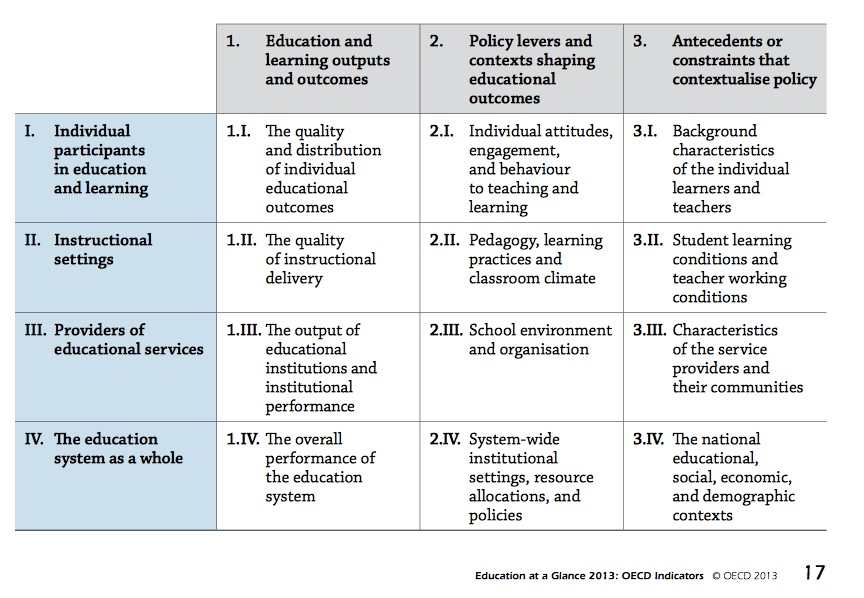
\includegraphics[width=13cm]{./images/oecdframe.jpg}
\center
\caption{Die ersten zwei Dimensionen des OECD Frameworks \cite[17]{oecd5} }
\end{figure}



Die Tabelle besteht aus drei Spalten und vier Zeilen. Die drei Zeilen unterscheiden die Akteure des Bildungssystemes. Dabei wird in den Zeilen von den ``individual participants '' also den individuellen Akteuren (Schüler,Lehrer etc.) bis hin zu einer ganzheitlichen Betrachtung des Systems aggregiert. Die Spalten bewerten zuerst das Ergebnis ``Education and learning outcomes'' und in den beiden anderen Spalten die aktuellen politischen Rahmenbedingungen(2. Spalte) und deren geschichtlichen Kontext (3.Spalte).

Die dritte Dimension sind dann die eigentlichen statistischen Erhebungen. Diese werden im OECD Kontext ``indicators'' genannt und beginnen mit dem dem Indikator A1.
Hierbei ist besonders zu beachten, dass ein Indikator zu mehreren Tabellenzellen zugeordnet werden kann. Genauso kann auch eine Tabellenzeile mehrere Indikatoren beinhalten.
Dieser komplexe Aufbau ist nötig um eine angemessene Messung der Bildung möglich zu machen. Leider wird keine Ergebniskennzahl bestimmt, um den Bildungsstand auf einen Blick erfassen zu können, dies liegt wahrscheinlich an der Komplexität des Verfahrens.
In dieser Arbeit werden einige der Indikatoren des Berichtes genutzt um ausgewählte Aspekte der Bildung international zu vergleichen. Für die nicht vorhandenen Länder wird versucht aus anderen Quellen entsprechende vergleichbare Zahlen zu finden.

\section{Vergleich ausgewählter allgemeiner Aspekte anhand ausgewählter Länder}

\subsection*{Bildungsausgaben}
Die folgende Auflistung zu den Bildungsausgaben (in Prozent des BIP) stammt aus: \cite[Indikator B4. S.219]{oecd5}. 
Die Auflistung der pro-Kopf-Ausgaben stammt aus der gleichen Publikation Indikator B1 S.174 Spalte: Primary to Tertiary Education.
Die Zahlen für Indien stammen aus: \cite[2]{oester}. Eine Übersicht über noch viele weitere Länder kann bei : \cite[165]{hdr} gefunden werden.

\begin{table}[htp]
\begin{tabular}{|c|c|c|c|c|c|}
\hline  	& Deutschland & USA & Indien  & Norwegen \\ 
\hline 	Prozent des BIP &4,8 & 5,5  & 3,3  & 8,8 \\ 
\hline  Pro-Kopf Ausgaben & ? & 15171 & m & 14081 \\ 
\hline 
\end{tabular} 
\caption{Bildungsausgaben, ? bedeutet fehlend.}
\end{table}
Aus dieser Auflistung ist deutlich zu erkennen, dass Deutschland im Verhältnis zu Indien im Verhältnis zum BIP wesentlich höhere Ausgaben für Bildung hat. Trotzdem existieren Länder wie Norwegen, in denen die Bildungsausgaben noch deutlich höher sind als in Deutschland. Es gibt also durchaus Steigerungspotential. In den USA entstehen die hohen Pro-Kopf Ausgaben auch dadurch, dass ein Großteil der tertiären Bildung privat finanziert werden muss (Studiengebühren für Colleges und Universities). 

\subsection*{Anteil der Erwachsenen die eine tertiäre Bildung genossen haben}
Diese Kennzahl ist geeignet um den Anteil an einer Altersgruppe zu ermitteln, die eine höhere berufsspezifische Bildung genossen haben. Darunter zählt in Deutschland ein Studium an einer Hochschule oder Berufsakademie oder einer Fachschule oder einer Fachakademie (Bayern). Wichtig um in diese Gruppe eingeordnet zu werden ist nach der allgemeinen Schulausbildung noch eine weitere abgeschlossene berufsspezifische Weiterbildung auf höherem Niveau.

\begin{figure}[H]
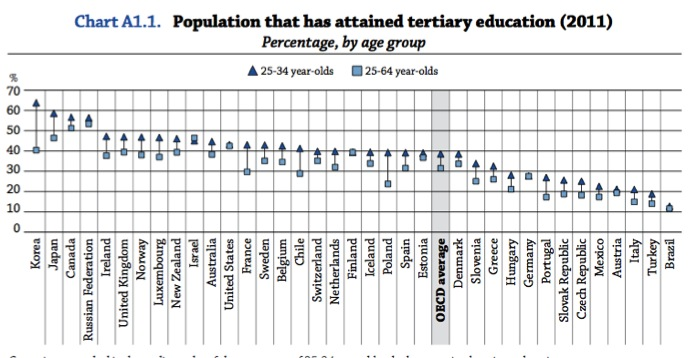
\includegraphics[width=15cm]{./images/tertiary.jpg}
\center
\caption{Anteil der Erwachsenen die eine tertiäre Bildung genossen haben. \cite[26]{oecd5} }
\end{figure}
Aus dieser Grafik lässt sich ableiten, dass für Deutschland in diesem Bereich mit knapp unter 30 \% großes Steigerungspotential vorhanden ist.
Am Beispiel von Korea kann man sehen, dass dort aktuell wesentlich mehr Menschen einen tertiären Bildungsabschluss besitzen. Dort sieht man auch, dass sich die Altersgruppen stark unterscheiden. Die 25-64 Jährigen liegen bei nur 40 \% die 25 bis 34 Jahre alten aber bei über 60 \%. In Deutschland ist kaum eine Veränderung zwischen den Altersgruppen zu erkennen.
Die USA liegen mit über 40 \% auch weit über deutschem Niveau. Auch dort ist zwischen den Altersgruppen fast keine Steigerung festzustellen.
Norwegen liegt auch knapp unter (ältere Gruppe) den USA, es ist aber eine Steigerung zwischen den Altersgruppen festzustellen. Es lässt sich die Schlussfolgerung treffen, dass die hohen tertiären Abschlussquoten in den USA und in Norwegen vielleicht in Zusammenhang mit den hohen Bildungsausgaben dieser Länder stehen.
Für Indien sind aus diesem Bericht keine Daten vorhanden.

\subsection{Besonderheiten ausgewählter Länder}
\subsubsection*{Deutschland}
Für Deutschland lässt sich eine steigende Studienanfängerquote feststellen. War diese 1995 noch bei 26 \%  stieg sie 2008 auf 36 \%  und 2009 auf 40 \% einer Altersgruppe. Dies liegt aber immer noch  weit unter dem OECD Schnitt von 59 \% .

Im Bericht `` Bildung auf einen Blick '' (Education at a glance) existiert auch eine Statistik, die die Absolventen einzelner Fächergruppen im Rahmen der OECD Länder vergleicht \cite{oecd3}. Demnach studieren deutsche Frauen eher `` Social Scienes, Business, Law '' und nur sehr wenige `` Engineering und Manufacturing Construction ''. In welches dieser Felder das IT-Consulting genau einzuordnen ist kann nicht beantwortet werden. Diese liegt auch daran, dass zum Beispiel in der Engineering Branche ein gewisser Bedarf an IT-Fachkräften besteht und deswegen auch Fachkräfte aus diesem Bereich kommen. Aus der Statistik auf Seite 83 der gleichen Veröffentlichung lässt sich auch erkennen, dass in Deutschland nur 23,6 \% der Studienanfänger ein Studium im Bereich `` Social Scienes, Business, Law '' aufnehmen. In Australien jedoch sind es 39,2 \% . Im ``Engineering,Manufacturing Construction'' Bereich hingegen ist Deutschland mit 15,2 \% im Mittelfeld vertreten, Australien kann hier nur  8,8 \% vorweisen. Die Studienanfängerquote für den Bereich Wirtschaftswissenschaften bietet also noch Steigerungspotenial in Deutschland im internationalen Vergleich.

Die OECD veröffentlicht auch jährlich die PISA Studie (Auszug der Ergebnisse für Deutschland: \cite{pisa} ). Hier wird die Bildungsqualität der einzelnen Mitgliedsländer anhand der Ergebnisse von Schülern miteinander verglichen. Die Studie von 2012 zeigt: Deutschland liegt mit seinen Ergebnissen in den Bereichen Mathematik, Naturwissenschaften und Leseverständnis im OECD-Durschnitt. Negativ fällt aber auf, dass Deutschland einen der höchsten Anteile an Sitzenbleibern im OECD Raum hat. Hier besteht Verbesserungspotential, vielleicht durch Veränderung des Bildungssystemes.

Wie bereits in der Einleitung erwähnt, existieren für Deutschland verschiedene Studienrichtungen, die sich speziell an Studenten richten, die ins Consulting wollen. Dies betrifft betriebswirtschaftliche Beratung (also Organisations- und Strategieberatung und HR-Beratung), für IT-Consulting gibt es fast keine entsprechenden Studienrichtungen oder Ausbildungen.
Eine Auflistung für diese ``allgemeinen'' Consulting Studiengänge liefert Nissen in seinem Werk: \cite{NissenKlaukDeelmannMohe201209}. 
Eine Ausnahme bildet die Studienrichtung ``IT-Management und -Consulting'' der Universität Hamburg, die sich auf das IT-Consulting beschränkt. Auch \cite{IDSScheer} beklagt einen Mangel an entsprechenden Studiengängen oder Ausbildungen.

Aus diesem Grund werden im Folgenden werden die Absolventenzahlen der Fächergruppen Rechts-, Wirtschafts- und Sozialwissenschaften und Ingenieurwissenschaften näher betrachtet.
Grundlage dafür bildet \cite{absolventen} . Durch die Bachelor/ Master Umstellung wird eine Aussage erschwert. Die Zahlen für nicht Bachelor/Master Abschlüsse sind stark rückläufig, dies liegt jedoch vor allem am Bologna Prozess und nicht am mangelnden Interesse der Wirtschaft. Das erkennt man daran, dass im gleichen Zeitraum die Absolventenzahlen sowohl für Wirtschaftswissenschaften, als auch für Ingenieurswissenschaften ansteigen (jeweils Bachelor und Master). Im Jahre 2012 haben sie ihren bisherigen Höchststand erreicht mit Rechts-, Wirtschafts- und Sozialwissenschaften 71.708 und 41.296 Absolventen in den Ingenieurwissenschaften (Bachelor).

Ob dieser Anstieg der Absolventen den Arbeitsmarkt genügend versorgt, ist schwierig zu ermitteln. Das liegt daran, dass geeignete Bedarfszahlen nicht gefunden werden konnten. Am Beispiel des so genannten Fachkräftemangels lässt sich gut das Problem der Erhebung solcher Bedarfszahlen nachvollziehen. Der von der Bitkom verbreitete Begriff \cite{fachkraft} des Fachkräftemangels wird von einigen Quellen bestritten, darunter zum Beispiel der Bundesagentur für Arbeit \cite{fachkraftnein}. Es existieren also mindestens zwei konkurrierende Ansichten die auch entsprechend verschiedene Ergebnisse veröffentlichen. Welche Zahlen geeigneter sind müsste durch eine intensive Auseinandersetzung mit dem zugrunde liegenden Ermittlungsverfahren herausgefunden werden.  In wie weit sich diese Zahlen für die gesamte IT-Branche auch speziell auf die IT-Consulting Branche beziehen lassen ist ebenfalls unklar.

\subsubsection*{USA}
Die USA kann im Vergleich zu Entwicklungsländern wie zum Beispiel Indien zu den Ländern mit dem höchsten Bildungsniveau gezählt werden. Dies bestätigt auch die Mitgliedschaft in der OECD. Das Bildungssystem der USA ist anders aufgebaut als das System in Deutschland. Es existiert keine Unterscheidung in Grund-/Mittel- Schule und Gymnasium. Die Kinder lernen unabhängig von ihren Leistungen miteinander bis zum High School Abschluss. Danach gibt es zwei Wege, für diejenigen die studieren wollen, Colleges und Universities. Colleges bilden eher praktisch aus und Universities eher forschungsorientiert, trotzdem existieren auch Colleges mit sehr hohem Ansehen in der Wirtschaft. 

Im Bericht ``Education at a glance '' der OECD (USA Country Notes: \cite{oecd4}) wird darauf hingewiesen, dass die Tertiary Education (Tertiäre Bildung, wird im allgemeinen Bildungsabschnitt beschrieben) stark davon abhängt ob die Eltern diese genossen haben. Dies liegt zum Teil auch an den enorm hohen Studiengebühren, die in den USA für das Studium in Colleges und Universities erhoben werden. Die wird auch dadurch unterstrichen, dass in den USA 62 \% der Aufwendungen für die tertiäre Bildung von Privat kommen. Der Durchschnitt aller OECD Länder ist nur 30 \%

In der letzten PISA Studie schnitt die USA insgesamt im Mittelfeld ab. In Mathematik lag Sie mit 481 Punkten knapp unter dem Durchschnitt von 494 Punkten der OECD. Die USA schnitt besser als 26 andere Staaten ab und schlechter als 29. \cite{pisa2}

\subsubsection*{Indien}

Die Bildungssituation in Indien unterscheidet sich wesentlich von der in Deutschland und der in den USA. Zwar wurde am 4. April 2009 eine gesetzliche Schulpflicht in der Verfassung festgeschrieben, doch es fehlen viele Lehrkräfte. \cite{dw} Die Bezahlung der Lehrer ist nur sehr gering und reicht oftmals nicht zum Überleben aus. Bildung gilt in Indien als Statussymbol, trotzdem können es sich viele Familien besonders auf dem Land nicht leisten. Dadurch resultiert eine sehr hohe Analphabetenrate \cite{analpha}. 2006 lag diese bei Männern bei 75,2 \% und bei Frauen bei 50,8 \% .
Trotzdem existieren in Indien einige technische Ausbildungseinrichtungen, die `` Indian Institutes of Technology '' die international mit den Spitzenuniversitäten mithalten können. Doch nur 10 \% der Schulabgänger die eigentlich studieren könnten, schaffen es auf die Unis. Viele Studenten zieht es nach ihrem Studium auch in die USA, Großbritannien oder Australien so das Indien viele potentielle Fachkräfte verliert.
Bildung ist also in Indien nicht selbstverständlich, sondern sehr kostbar. Nur wenige Ausbildungseinrichtungen lehren auf europäischem oder amerikanischem Niveau. Demnach existiert aufgrund der sehr großen Bevölkerungszahl ein hohes Potential an möglichen Fachkräften, falls sich das Bildungssystem grundlegend ändert.

Der Bericht des DAAD (Deutscher Akademischer Austauschdienst) \cite{daad} wird erneut ein Mangel an Lehrenden beklagt nur 30-40 \% der Stellen seien besetzt (S.96).
Studiengebühren werden, für europäische Verhältnisse, in eher geringem Maß erhoben. Aufgrund des viel geringeren Durchschnittseinkommens sind diese jedoch ein Hindernis für viele Studierwillige. Das Durchschnittseinkommen beträgt ca. 1.022 Euro \cite{ausa} die Studiengebühren je Jahr reichen von 50 an staatlichen Hochschulen bis 12.000 Euro an privaten Institutionen \cite[101]{daad}.


 \section{spezielle Aspekte}
Dieser Teilabschnitt bezieht sich im Gegensatz zum eher allgemeinen Abschnitt Bildung stärker auf das IT-Consulting. Es werden verschiedene Teilaspekte beschrieben, die einen stärkeren Bezug zum IT-Consulting haben. Da aber oftmals keine spezifischen Daten zu IT-Consulting Studiengänge oder Ausbildungen vorhanden sind (da es oft keine allgemein anerkannten Ausbildungen für diese Branche gibt) wird mit verschiedenen Fächergruppen gearbeitet, in die IT-Consulting eingeordnet werden soll. 
Dadurch ergibt sich das Problem der Einordnung von IT-Consulting in die Fächergruppen Ingenieurwissenschaften und Wirtschaftswissenschaften/Rechtswissenschaften. Durch den interdisziplinären Charakter des IT-Consultings ist eine genaue Zuordnung nicht möglich. Trotzdem kann man anhand der Absolventenzahlen bestimmte Schlussfolgerungen ziehen und somit den potenziellen Arbeitnehmermarkt charakterisieren.

Nachfolgend eine (unvollständige) Liste einiger Teilaspekte die zur Einschätzung des Arbeitnehmermarktes eines Landes in Bezug auf die IT-Consulting relevant sind. 
\begin{itemize} 
\item Welche IT-Consulting Studiengänge existieren?
\item Welche anderen Studiengänge sind für IT-Consulting relevant?
\item Wie viele Absolventen gibt es in den relevanten Studiengängen?
\item Welche anderen Ausbildungsformen existieren für IT-Consulting?
\item Welches Wissen benötigen IT-Consultants? Wird dieses angemessen vermittelt?
\item Wie ist die Qualität der IT-Ausbildung im jeweiligen Land?
\item Forschung
\item ...
\end{itemize}

Einige dieser Aspekte und ihre Relevanz für das IT-Consulting werden im Folgenden erläutert.

\subsection*{Relevante Studiengänge}
Wie bereits erwähnt ist es aufgrund des interdisziplinären Charakters des Faches schwierig, IT Consulting zu einem Studienbereich oder einem Studiengang zuzuordnen. 
In Deutschland existieren vereinzelt aber auch Bachelor und Masterstudiengänge, die Consulting im Namen als Bestandteil haben, so z.B. der Master Studiengang ``IT-Management und -Consulting'' der Universität Hamburg. Ein genauerer Überblick über die in Deutschland, Österreich und der Schweiz verfügbaren spezifischen Bachelor Studiengänge wird in \cite{NissenKlaukDeelmannMohe201209} gegeben. Trotzdem stellen die Absolventen dieser speziellen Studiengänge nur einen kleinen Teil der benötigten Fachkräfte dar.

Es erscheint logisch, das die Studienrichtung Wirtschaftsinformatik durch die interdisziplinäre Ausrichtung gut zum IT-Consulting passt. Auch die Studiengänge Betriebswirtschaftslehre sowie Informatik sind, aufgrund der Studieninhalte, für eine IT Consulting Karriere geeignet. Wie verschieden die Ausbildungswege sind die ins Consulting führen lässt sich nur schwer ermitteln, das keine Statistiken über die Herkunft der Berufseinsteiger im IT-Consulting gefunden werden konnten.
So ist zum Beispiel sicherlich auch denkbar, dass ein Absolvent der Volkswirtschaftslehre bei entsprechendem IT-Vorwissen zum Vorstellungsgespräch eingeladen wird, genauso aber auch ein Absolvent eines technischen Studienganges (zum Beispiel Informationstechnik), der sich betriebswirtschaftlich weitergebildet hat.

\subsection*{Absolventen in relevanten Studiengängen}
Dieser Teilaspekt setzt natürlich eine Auswahl an relevanten Studiengängen oder Ausbildungen voraus. Die Anzahl der Absolventen wäre dann die potentielle Menge die dem Arbeitsmarkt zur Verfügung stehen würde. Werden besonders viele ausländische Fachkräfte für die Beratung eingestellt, kann man auf einen Mangel an eigenen ausgebildeten Fachkräften schließen und somit auf einen höheren Bedarf an die Ausbildungseinrichtungen in diesem Land.

\subsection*{Forschung}
Der Bereich Forschung beschreibt die für das IT-Consulting relevanten Forschungsaktiväten und Ergebnisse. Wiederrum ist es schwierig eine genaue Zuordnung von Forschungsaktivitäten in verschiedenen Fakultäten zur Beratungsbranche zu treffen. Zu diesem Teilaspekt besteht der größte Forschungsbedarf, da bisher nur wenig relevante wissenschaftliche Forschung betrieben wird.\cite[10]{nissen2007consulting},\cite{IDSScheer}[1]

Einige Teilaspekte zur Forschung sind beispielsweise:
\begin{itemize}
\item Verhältnis Forschung zur Praxis im IT-Consulting
\item Anzahl der wissenschaftlichen Veröffentlichungen die das IT Consulting betreffen
\item Forschungsgelder und Subventionen
\item ...
\end{itemize}

Einige dieser Aspekte und ihre Relevanz für das IT-Consulting werden im Folgenden erläutert.

\subsubsection*{Anzahl der wissenschaftlichen Veröffentlichungen}
Dieser Teilaspekt betrifft die Anzahl der wissenschaftlichen Veröffentlichungen, die sich mit IT-Consulting beschäftigen. 
Für Deutschland existiert eine vom statistischen Bundesamt veröffentliche Erhebung zur Anzahl und Fächerverteilung der Promovierenden.\cite{destatis}
Auch bei dieser Statistik ergibt sich, dass eine exakte Aussage nicht möglich ist. Trotzdem kann man
von den Fächergruppen eine Aussage ableiten, diese ist dann zwar nicht absolut sicher, bietet aber eine Grundlage.

\subsubsection*{Verhältnis Praxis zu Forschung}
In verschiedenen Veröffentlichungen zum Beispiel: \cite[1]{IDSScheer} wird ein Mangel an ``Grundlagenforschung'' und ``Modelltheorien'' festgestellt. Es existiert jedoch auch die Forschungsrichtung ``Consulting Research'' (Volker Nissen). Diese stellt zwar einen Forschungsansatz für das betriebswirtschaftliche Consulting dar, jedoch kommt auch die IT-Beratung darin vor. Consulting Research besitzt laut Nissen zwei Ziele: ``Erstens, die wissenschaftliche Durchdringung des Themas Unternehmensberatung, wobei der von einzelnen Beratungsprojekten abstrahierende wissenschaftliche Erkenntnisgewinn im Mittelpunkt steht. Zweitens, die Übertragung wissenschaftlicher Theorien, Erkenntnisse und Methoden auf die unternehmerische Praxis mit dem Ziel, Aufgabenstellungen und Probleme im Umfeld von Beratungsprozessen und Beratungsunternehmen besser als bisher zu lösen.''
(Ausführliche Diskussion des Verhältnisses von Praxis zu Theorie auf S.23 ff)

Nissen erkennt auch ein „ Defizit an wissenschaftlicher Auseinandersetzung [...] mit Themen der IT-orientierten Beratung“. Dies erschwert es eine Aussage zum Forschungsstand im IT-Consulting zu treffen.

\subsubsection*{Staatliche Forschungsgelder/Subventionen/Zuschüsse}
Dieser Teilaspekt beschäftigt sich mit der Höhe der Forschungsgelder, die dem IT-Consulting zugeordnet werden können. Durch höhere Forschungsgelder können mehr Forscher eingestellt werden und mehr Zeit investiert werden, dies kann zu einer höheren Qualität der Ergebnisse führen. Forschungsgelder sind demnach relevant sowohl für die Menge der Forschungsarbeiten als auch für deren Qualität.
Für Deutschland existieren z.B. Statistiken die staatliche Forschungsgelder nach Fakultäten auflistet (sowohl für Universitäten als auch für Fachhochschulen) \cite {ausgabenfakuni}, \cite {ausgabenfakfach}, \cite {ausgabenbmbf}. Erneut ist die Zuordnung des IT-Consultings zu einem der Fachbereiche Ingenieurwissenschaften (in der dritten Statistik stellt Informatik ein eigenes Fach dar) oder Wirtschafts-/Rechtswissenschaften nicht mit absoluter Sicherheit möglich.

\section{Vergleich ausgewählter spezieller Aspekte anhand ausgewählter Länder}

\subsection*{Eingeschriebene Studenten in relevanten Studiengänge}
In der folgenden Statistik wird ein Vergleich der in bestimmten Fächergruppen eingeschriebenen Studenten anhand verschiedener Länder vorgenommen. Da es die Fächergruppe IT-Consulting beziehungsweise Informatik in den ausgewählten Statistiken nicht gibt werden die beiden Fächergruppen Ingenieurwissenschaften und Wirtschaftswissenschaften benutzt. Es wurde jedoch auch eine Statistik gefunden, in der Computing als einzelne Fachrichtung angegeben wird. Dabei werden alle relevanten Studierenden mitgezählt also sowohl Bachelor/Master/Diplom/Promotion aber auch zum Beispiel in den USA Graduates und Undergraduates sowie PhD Studierende.
Die Zahlen für Deutschland, USA, Norwegen, Großbritannien und Frankreich stammen aus: \cite{studierende} (Der Data Explorer muss mit einigen Optionen angepasst werden um die gewünschten Statistiken anzuzeigen) und sind von 2011. Die Zahlen für Indien sind von 2005 und stammen ebenfalls vom BMBF : \cite{indienstudierende} .

\begin{table}[htp]
\begin{tabular}{|p{3cm}|c|c|c|c|c|c|}
\hline  	& Deutschland & USA & Indien  & Norwegen & GB & Fr \\ 
\hline  Business and administration & 419,553 & 3,490,011  & 1.986.146  & 36,090 & 321,750 & 422,201 \\ 
\hline  Engineering, manufacturing and construction & 492,122 & 1,522,722 & 795.120 & 18,691 & 211,948 & 299,153 \\ 
\hline  Computing &141,625  & 642,308 &? & 8,288 & 98,714 & 70,974\\ 
\hline 
\end{tabular} 
\end{table}
Die Statistik beschreibt die Anzahl der Studenten die in den jeweiligen Fachbereichen im jeweiligen Land eingeschrieben sind. Deutlich ist zu erkennen, dass Deutschland im Computing Bereich fast doppelt so viele Absolventen besitzt wie Frankreich. Die USA liegen in diesem Bereich jedoch mit dem 4,5 fachen der der deutschen Studenten sehr weit vorne. Dabei darf man natürlich nicht außer Acht lassen, dass die USA wesentlich größer ist als Deutschland und mehr Hochschulen besitzt.







